%
\section{Parton distribution functions\protect\footnote{
  S. Forte, J. Huston, K. Mazumdar, R.S. Thorne and A. Vicini.}}
\label{pdfsection}


\subsection{Introduction}
\label{intro}

Parton distribution functions (PDFs) are crucial for the prediction
of any physical process to be measured at the LHC, hence PDFs and their
uncertainties 
 have very important significance, in particular for discovery and
 exclusion limits. 
At present these PDFs are obtained 
from fits to data from deep-inelastic scattering, Drell--Yan, and
jet production from a wide variety of different experiments. 
A number of groups have produced publicly available PDFs
using different data sets and analysis frameworks. Here we 
summarise our level of understanding as the first LHC cross sections
at $7$\UTeV\ are being determined.  There are many differences between
existing PDF analyses: different input data, different methodologies and 
criteria for  determining uncertainties, different ways of 
parametrizing the PDFs, different
number of parametrized PDFs, different treatments of heavy quarks, 
different perturbative orders,
different ways of treating  $\alphas$ (as an input or as a fit
parameter),
different values of physical parameters such as $\alphas$ and
heavy-quark masses, and more. 
Hence, we begin by summarizing the main features of
current PDF sets. We subsequently introduce various
theoretical uncertainties on PDFs, focusing on the uncertainty related to
the value of the strong coupling constant, and provide a presentation
of choices made by different groups. We then briefly 
summarise the computation of physical processes using various PDF sets. 
As an outcome of this, we motivate and 
describe the PDF4LHC interim recommendation~\cite{PDF4LHCwebpage} 
to obtain current combined predictions and uncertainties based on several 
global PDF sets, and illustrate it by showing its
application to the  Higgs production 
cross section via gluon--gluon fusion, both at
NLO and at NNLO. 

\begin{sloppypar}
We will discuss the following PDF sets (when several
releases are available, the reference release for our discussion below 
is given 
parenthesis in each case):
ABKM~\cite{Alekhin:2009ni}, CTEQ/CT (CTEQ6.6~\cite{Nadolsky:2008zw}),
GJR~\cite{Gluck:2007ck,Gluck:2008gs}, HERAPDF (HERAPDF1.0~\cite{:2009wt}), 
MSTW (MSTW08~\cite{Martin:2009iq,Martin:2009bu,Martin:2010db}) and 
NNPDF (NNPDF2.0~\cite{Ball:2010de}). ABKM, JR~\cite{JimenezDelgado:2008hf}
(for variable flavour see \Bref{JimenezDelgado:2009tv}), 
MSTW, and HERAPDF~\cite{CooperSarkar:2010ik} are 
available with NNLO evolution \cite{Moch:2004pa,Vogt:2004mw}.
A CTEQ/CT update is already
available (CT10~\cite{Lai:2010vv}),  while preliminary updates of
ABM~\cite{Alekhin:2010iu}, NNPDF~\cite{Rojo:2010gv},
HERAPDF~\cite{CooperSarkar:2010ik},
 and
MSTW~\cite{Thorne:2010kj} have also been presented.
\end{sloppypar}


\subsection{PDF determinations -- experimental uncertainties}
\label{sec:pdfdet1}

Experimental uncertainties on PDFs determined in global fits (usually 
called {\em PDF uncertainties}, for short) reflect the information available 
(or lack thereof) in the underlying data and the way it constrains PDFs; they
should be
interpreted as genuine statistical uncertainties, and indeed they are often
given in the form of confidence levels (CL). 
They may differ because of different choices made in the analysis
that extracts this information from the data, specifically in: 
(1) the choice of data sets; (2) the statistical
 treatment which is used to determine the uncertainties and which also
determines the way in which PDFs are delivered to the user; (3) the
form and size of parton parametrization. 


\subsubsection{Data sets}
\label{data}
A wider data set contains more information, but data coming
from different experiments may be inconsistent to some extent. The
choices made by the various groups are the following:
\begin{itemize}
\item The data sets considered by CTEQ, MSTW, and NNPDF include data from both  
electroproduction 
and hadroproduction, in each case from both
  fixed-target and collider experiments. The electroproduction data
  include electron, muon and neutrino  
 deep-inelastic scattering data (both inclusive and charm
 production). The hadroproduction data include Drell--Yan (fixed-target
 virtual photon and collider $\PW$ and $\PZ$ production) and jet
 productions (Tevatron jets requiring some approximation for the MSTW NNLO
analysis). 
Details vary slightly among particular versions of CTEQ, MSTW, and NNPDF 
fits. 
\item For GJR (and JR) the data set consists of electroproduction data 
which include electron- and muon-inclusive
 deep-inelastic scattering data, and deep-inelastic charm 
 production from charged leptons and neutrinos from
  fixed-target and collider experiments, and a smaller set of 
hadroproduction data, i.e.\ fixed-target virtual photon Drell--Yan 
production and  Tevatron jet production.
\item The ABKM data set includes electroproduction  from
  fixed-target and collider experiments, including electron, 
muon, and neutrino deep-inelastic scattering data (both inclusive and charm
 production), and fixed-target hadroproduction data, i.e.\ virtual
 photon Drell--Yan production%
\footnote{An update is being prepared that includes the Tevatron jet data as well.}. 
\item The HERAPDF input contains all HERA deep-inelastic inclusive
data.   
\end{itemize}

\subsubsection{Statistical treatment}
\label{stat}

Available PDF determinations fall in two broad categories: those
based on a Hessian approach and those which use a Monte Carlo
approach. The output format for information on PDFs is different in 
each case. Here we  outline only the basic features. The precise manner 
in which to implement the PDFs 
is explained in more detail in the appropriate 
references for each group. 

Within the Hessian method, PDFs are determined by minimizing a
$\chi^2$ function defined as
  $\chi^2=\frac{1}{N_{\rm dat}}\sum_{i,j}
  (d_i-\bar d_i){\rm cov}_{ij}(d_j-\bar d_j)$, where $\bar d_i$ are data,
  $d_i$ theoretical predictions, ${N_{\rm dat}}$
  is the number of data points,
%(note the inclusion of the factor  $\frac{1}{N_{\rm dat}}$ in the definition) 
and ${\rm cov}_{ij}$ is
  the covariance matrix%
\footnote{Different groups use differing
  definitions of the covariance matrix -- including entirely or only
  partially correlated uncertainties -- see the papers for details. 
  Hence the values of the $\chi^2$
  quoted are only roughly comparable.}. 
The best fit is the point in parameter
space at which $\chi^2$ is minimum, while PDF uncertainties are found
by evaluating, and often diagonalizing the (Hessian) matrix of second
derivatives of the $\chi^2$ at the minimum, and then 
%(see Fig.~\ref{fig:hessian}) 
determining the range of parameter variation 
corresponding to a  prescribed
increase of the $\chi^2$ function with respect to the minimum.
In principle, the increase in $\chi^2$ which provides
$68\%$~CL  ($1 \,\sigma$) is $\Delta\chi^2=1$.  However, a larger variation
of $\Delta\chi^2=T^2$, with $T>1$  a suitable `tolerance'
 parameter~\cite{Stump:2001gu,Pumplin:2001ct,Martin:2002aw} may
turn out to be necessary for a more realistic error estimate for fits
containing a wide variety of input processes and data, and 
in particular, in order for each
 experiment which enters the global fit to be consistent
 with the global best fit within one sigma (or an alternative
 confidence level, 
e.g.\ $90\%$).  Possible reasons why this is necessary could be 
data inconsistencies or incompatibilities, 
underestimated experimental systematics, insufficiently flexible
parton parametrizations, theoretical uncertainties or approximations in
the PDF extraction. At present, HERAPDF and ABKM use $\Delta\chi^2=1$,
GJR uses $T\approx4.7$, CTEQ6.6
uses $T=10$ at $90\%$ ~CL (corresponding to $T\approx6$ at $68\%$~CL), while MSTW08 uses a dynamical tolerance~\cite{Martin:2009iq}, i.e.,\ a different value
of $T$ for each eigenvector, with values 
%{\bf 
%for one sigma
%}
from $T\approx 1$ to
$T\approx 6.5$ and most values being in the range of $2<T<5$. 

Within a Monte Carlo method, PDFs are determined by first producing a
Monte Carlo sample of $N_{\rm rep}$ pseudo-data replicas. Each replica
contains a number of points equal to the number of original data
points.
 The sample is constructed
in such a way that, in the limit $N_{\rm rep}\to\infty$, 
the central value of the $i$-th
data point is equal to the mean over the $N_{\rm rep}$ values that the
$i$-th point takes in each replica,  the uncertainty of the
same point is  equal to the variance over the
replicas, and the correlations between any two original data
points is equal to their covariance over the replicas. From 
each pseudo-data replica, a PDF replica  is constructed by minimizing
a $\chi^2$ function. The PDF
central values, uncertainties and correlations are then computed by
taking means, variances, and covariances over this replica
sample. NNPDF uses a Monte Carlo method, with each PDF replica
obtained as the minimum $\chi^2$ which satisfies a cross-validation
criterion~\cite{Ball:2008by,Ball:2010de}, and is thus larger than the
absolute minimum of the $\chi^2$. This method has been used in all NNPDF sets
from NNPDF1.0 version onwards. 
%{\it (Fair to mention this has evolved from set to set?)}

\subsubsection{Parton parametrization}
\label{parm}
Existing PDF sets differ in the number and choice of linear combinations 
of PDFs which are independently parametrized and the functional form and 
number of parameters used.
For the functional form the most common choice is that
each PDF at some reference scale $Q_0$ is parametrized as
\beq
f_i(x,Q_0)=N x^{\alpha_i} (1-x)^{\beta_i} g_i(x)
\label{pdfparm}
\eeq
where $g_i(x)$ is a function which tends to a constant for both $x\to1$
and $x\to0$, for example $g_i(x)=1+ \epsilon_i \sqrt{x}+ D_i x+ E_i x^2$ (HERAPDF). The fit parameters are $\alpha_i$, $\beta_i$, and the
parameters in $g_i$. Some of these parameters may be chosen to take a
fixed value (including zero).
The general form (\ref{pdfparm})  is adopted in
all the PDF sets which we discuss here except for the case of NNPDF which, instead, defines
\beq
f_i(x,Q_0)= c_i(x) NN_i(x),
\label{pdfparmnn}
\eeq
where $NN_i(x)$ is a neural network (a feed-forward neural network
with two hidden layers, see
\Bref{Ball:2010de} for details)
%(a 2-5-3-1 feed-forward neural network for NNPDF2.0), 
and $c_i(x)$ is  a
{\em preprocessing} function. The fit parameters determine the shape 
of $NN_i(x)$. The function $c_i(x)$
is chosen randomly in a space of functions of
the form $x^{\alpha_i} (1-x)^{\beta_i}$, within some acceptable range of
the parameters $\alpha_i$ and $\beta_i$.
For each group the basis functions and number of parameters are the following.

\begin{itemize}
  
\item ABKM parametrizes the two lightest flavours, corresponding
  anti-flavours, the total strange-ness, and the gluon (six independent
  PDFs) with 21 free parameters.
\item CTEQ6.6 and CT10  parametrize  the two lightest flavours and
  anti-flavours, the total strangeness, and the gluon (six independent
  PDFs) with respectively $22$ and $26$ free parameters.
\item GJR parametrizes the two lightest flavours, their anti-flavours,
  and the gluon with $20$ free parameters (five independent PDFs); the
  strange distribution is assumed to be either proportional to the
  light sea or to vanish at a low scale $Q_0<1$\UGeV\ at which PDFs become valence-like.
\item HERAPDF parametrizes the two lightest flavours, $\PAQu$,
  the combination $\PAQd + \PAQs$, and the gluon with $10$ free
  parameters (five independent PDFs), strangeness is assumed to be
  proportional to the $\PAQd$ distribution; the
  effect of varying the form of the parametrization and the  
  size of the strange component is also studied.  
\item  MSTW parametrizes the three lightest flavours and anti-flavours, and
  the gluon with $28$ free parameters (seven independent PDFs) to find
  the best fit, but $8$ are held fixed in the determination of the uncertainty eigenvectors.
\item NNPDF parametrizes the three lightest flavours and
  anti-flavours, and the gluon with $259$ free parameters ($37$ for
  each of the seven independent PDFs).

\end{itemize}


\subsection{PDF determinations -- theoretical uncertainties}
\label{sec:pdfdet2}


The theoretical uncertainties of the PDFs
reflect the approximations in the theory
which is used in order to relate the PDFs to the measurable quantities.
The study of theoretical PDF uncertainties is currently less advanced
than that of  experimental uncertainties, and only some of
the theoretical
uncertainties have been explored till now. One might expect that one of 
the main theoretical uncertainties in PDF determinations
should be related to the treatment of the strong interaction: in
particular, to the values of the strong coupling constant ($\alphas$) 
and of the heavy-quark masses  ($\Mc$ and
$\Mb$), and the uncertainties related to the truncation of the perturbative
expansion (commonly estimated through the variation of renormalization
and factorization scales). The uncertainty on $\alphas$ has
been explored systematically by the PDF groups. The  effect of varying $\Mb$ and
$\Mc$ has been included by HERAPDF in  
model uncertainties, and these are parameters in the covariance matrix for 
ABKM~\cite{Alekhin:2009ni}. Sets with varying quark masses 
and implications have been 
made available by MSTW~\cite{Martin:2010db}, and 
preliminary studies of the effect of $\Mb$ and $\Mc$ have also been 
presented by NNPDF~\cite{Guffanti:2010yu}.
 Further uncertainties are related to the
treatment of the heavy-quark thresholds, which are handled in various ways
by different groups (see Section~22 of \Bref{Binoth:2010ra}), 
to numerical approximations,
and to the treatment of electroweak effects (such as QED PDF evolution~\cite{Martin:2004dh}).

\subsubsection{The value of $\alphas$ and its uncertainty}

The choice of value of $\alphas$ is clearly important because it
is strongly correlated to PDFs, especially the gluon distribution: this
correlation is studied in detail in \Bref{Demartin:2010er} using
CTEQ, MSTW, and NNPDF PDFs; 
$\alphas$ is a parameter in the covariance matrix for 
ABKM, GJR(JR). 
There are two separate issues related to the value of $\alphas$ in
PDF fits: first, the choice of $\alphas$ for which PDFs are made available, and second the choice of the preferred value of $\alphas$ to be
used when giving PDFs and their uncertainties. 
These are  two separate though related issues, and for each of them
two different basic philosophies 
may be adopted. In what concerns available  values, 
for some groups PDF fits 
are performed for a number of different values of
  $\alphas$. Though a  PDF set corresponding to some
  reference value of $\alphas$ is given, the user is free to
  choose any of the given sets. This philosophy is adopted by CTEQ ($0.118$),
  HERAPDF ($0.1177$), MSTW ($0.120$), and NNPDF ($0.119$), where, in parenthesis, the reference (NLO) value of $\alphas$ for each set is indicated.
  For others, $\alphas$ is treated as a fit parameter, and PDFs
  are given only for the best-fit value. This philosophy is adopted
  by ABKM ($0.11801$) and GJR ($0.1145$).
Concerning the preferred central value and uncertainty, 
for some groups the value of 
$\alphas(\MZ)$ is taken as an external parameter. 
  This philosophy is adopted by CTEQ,
  HERAPDF1.0, and NNPDF. In this case, there is no a-priori central value of $\alphas(\MZ)$, and the uncertainty on
  $\alphas(\MZ)$ is included by repeating the PDF determination as
  $\alphas$ is varied in a suitable range. 
  For others $\alphas$ is treated as a fit parameter, so its value
  and  uncertainty are
  determined along with the PDFs. This  philosophy is adopted by
  MSTW, ABKM, and GJR08.
%Concerning the preferred central value and the  
%treatment of the $\alphas$ uncertainty, the methodology varies. For CTEQ,
%  HERAPDF1.0  and NNPDF the value of 
%$\alphas$ is taken as an external parameter. 
%  In this case, there is no a-priori central value of $\alphas$ and the uncertainty on
%  $\alphas$ is treated by repeating the PDF determination as
%  $\alphas$ is varied within a suitable range. 
%  For MSTW, ABKM and GJR08 the value of $\alphas$ and its uncertainty 
%  are treated as fit parameters, and
%  determined along with the PDFs. For  ABKM and GJR08
% the uncertainty on 
%$\alphas$ is part of the Hessian matrix of the fit
%As a cross-check,~\cite{Lai:2010nw} CTEQ has also used the 
%world average value of $\alphas(M_Z^2)$ 
%as an extra input to the global fit.
%
%
%\begin{figure}
%\begin{center}
%\includegraphics[height=65mm,angle=0]{alphaSMZ68cl_updated.eps}
%\caption{\label{fig:alphas}  
%Values of $\alphas(M_Z^2)$ for which fits are available. The 
%default values and uncertainties used by each group are also shown.
%Plot by G. Watt \cite{Watt}.}
%\end{center}
%\end{figure}



%The values of $\alphas(M_Z^2)$ for which fits are available, as well as
%the default values and uncertainties used by each group are 
%summarized in Fig.~\ref{fig:alphas}.  
%The most recent world average value of $\alphas(M_Z^2)$ is
% $\alphas = 0.1184\pm0.0007$~\cite{Bethke:2009jm}. However, a more
%conservative estimate of the uncertainty on $\alphas$ was felt to be
%It may not be unreasonable to argue that a a yet 
%larger uncertainty may be appropriate. 

%{\bf We also note that the values used in the average are from extractions 
%at different orders in the perturbative expansion.}


When comparing results obtained using different PDF sets it should be
borne in mind that if different values of $\alphas$ are used,
 predictions for cross sections change both due to their dependence on 
$\alphas$ (which for some LHC processes,
such as top-pair production or Higgs 
production in $\Pg\Pg$ fusion may
be quite strong), as well as to the dependence of the PDFs on the
value of $\alphas$. Differences due to the PDFs alone can be isolated
only while performing comparisons at a common value of $\alphas$. The
different groups have different ways of calculating the total uncertainty 
due to both the PDFs and $\alphas$. This is explained in more detail 
in \Bref{Demartin:2010er}  and in publications from each of the groups, in 
particular, \Brefs{Martin:2009bu,Lai:2010nw,Alekhin:2009ni}.  




\subsection{Comparison of results from different PDFs}
\label{sec:benchmarking}

To compare results from different PDF sets it is useful to introduce 
differential parton--parton luminosities, which, when multiplied by the 
dimensionless cross section $\hat{s}\hat{\sigma}$ for a process, 
provide an estimate  of 
the size of an event cross section at the LHC. 
The differential parton--parton luminosity $dL_{ij}/d\hat{s}$ is
\begin{equation}
\frac{d L_{ij}}{d\hat{s}\,dy} \equiv 
\frac{1}{s} \, \frac{1}{1+\delta_{ij}} \, 
[f_i(x_1,\mu) f_j(x_2,\mu) + (1\leftrightarrow 2)] \; ,
\label{eq1}
\end{equation}
where the prefactor avoids double-counting for identical partons. A 
generic cross section is written as
\begin{equation}
\sigma = \sum_{i,j} \int_0^1 dx_1 \, dx_2 \, 
f_i(x_1,\mu) \, f_j(x_2,\mu) \, \hat{\sigma}_{ij}
\equiv \sum_{i,j} \int \left(\frac{d\hat{s}}{\hat{s}} \right) 
\, \left(\frac{d L_{ij}}{d\hat{s}}\right) \, 
\left(\hat{s} \,\hat{\sigma}_{ij} \right) \; .
\label{eq:xseclum}
\end{equation}



\begin{figure}[ht]
\begin{center}
%\includegraphics[width=0.48\textwidth]{fig1.eps}
%\includegraphics[width=0.48\textwidth]{fig2.eps}\\
\includegraphics[width=0.48\textwidth]{YRHXS_PDF/YRHXS_PDF_1.eps}
\includegraphics[width=0.48\textwidth]{YRHXS_PDF/YRHXS_PDF_2.eps}
\vspace{-0.8cm}
\caption{\label{fig:gglum} The $\Pg\Pg$  
luminosity functions and
uncertainties at $7$\UTeV, normalized to the MSTW08 result. 
(Plots by G.~Watt~\cite{Watt}.)}
\vspace{-0.6cm}
\end{center}
\end{figure}


The relative $\Pg\Pg$ PDF luminosities at NLO, along with their $68\%$~CL
error bands, are shown in \Fref{fig:gglum},
normalized to the MSTW08 central value~\cite{Watt}.
For HERAPDF1.0 the inner uncertainty bands (dashed lines) 
correspond to the experimental errors, and the
outer uncertainty bands (shaded regions) include errors due to model and
parametrization. The $\PQq\PAQq$ luminosity plots \cite{Watt} look 
similar, but turn upwards at high $\hat s/s$ for HERAPDF1.0. The error 
bands for each of the PDF
luminosities are of similar size. The luminosity  for the range of 
$\PQt\PAQt$ and Higgs production  are in
good agreement for CTEQ, MSTW, and NNPDF, while the agreement
with ABKM, HERAPDF, and GJR is less good at higher masses. 
%(Note however that these plots do not illustrate the effect that 
%the different $\alphas(M_Z^2)$ values used by different groups will have 
%on (mainly) $t\bar{t}$ and Higgs cross sections.)
It is notable that the PDF
luminosities tend to differ at low $x$ and high $x$. 
The CTEQ6.6 distributions, for
example, may be larger at low $x$ than MSTW2008, due to the
positive-definite parametrization of the gluon distribution; the MSTW
gluon starts off as negative at low $x$ and $Q^2$, and this results in an
impact for both the gluon and sea-quark distributions at larger $Q^2$
values. The NNPDF2.0 $\PQq\PAQq$ luminosity tends to be somewhat lower,
in the $\PW,\PZ$ region for example.  Part of this effect might come from
the use of a zero-mass heavy-quark scheme, although other differences 
might be relevant. However, there are other discrepancies of more than $20\%$
at high or low invariant masses. 

At small $x$ details of heavy-flavour 
treatment cause some deviation, and there is also an 
anticorrelation with the value of $\alphas$ which varies 
between groups (with the GJR value differing most). 
At high $x$ Tevatron jet data gives a constraint on the gluon 
(though there is some variation depending on the data set) 
and this data is not used in ABKM09 (investigations by ABM may be found at 
\Brefs{Trento,PDF4LHCnov10}) and 
HERAPDF1.0 fits. At high $x$, $\PW$ production data (not used by ABKM,
GJR, and HERAPDF) 
constrain the light-quark distributions, which are then correlated to
the gluon by the momentum sum rule.
 The high and low-$x$ gluon distributions are also 
anti-correlated by the momentum sum rule. All these factors, amongst
others, may influence the forms of the gluon luminosities and be
responsible for the discrepancies observed.
   
Benchmark computations of LHC total 
cross sections and rapidity distributions from various PDF groups
can be found in~\Bref{PDF4LHCwiki}
(see also \Bref{Alekhin:2010dd});  the degree of agreement and 
discrepancy between the groups is commensurate with the luminosity plots 
shown here. Differences between the luminosities and predictions 
for those sets which exist at NNLO are similar to NLO, showing that 
they are most likely due to choices of data sets in the fit or other assumptions 
rather than theoretical procedures, such as 
different schemes for the treatment heavy flavours, 
for which differences should become smaller at higher orders.

\begin{figure}
  \begin{center}
    \includegraphics[width=0.48\textwidth]{YRHXS_PDF/YRHXS_PDF_3.eps}
    \includegraphics[width=0.48\textwidth]{YRHXS_PDF/YRHXS_PDF_4.eps}\\
\vspace{-0.2cm}
\includegraphics[width=0.48\textwidth]{YRHXS_PDF/YRHXS_PDF_5.eps}
\vspace{-0.6cm}
\caption{\label{fig:Higgscs} Cross-section predictions as a function
  of $\alphas$ for a Higgs 
($\Pg\Pg$ fusion) for a Higgs mass of $120$\UGeV\ at NNLO for the 
Tevatron and LHC at $14$\UTeV~\cite{Martin:2009bu} (top-left)  
and at NLO for the LHC at $7$\UTeV~\cite{Ubiali:2010xc} (top-right) and for 
various groups all at NLO~\cite{Ubiali:2010xc} (bottom).}
\vspace{-0.6cm}
\end{center}
\end{figure}

It is also very useful to show the cross sections as a
function of $\alphas$.
The predictions for Higgs production  from $\Pg\Pg$ fusion
(shown for MSTW08 and NNPDF2.0 in the top left and right plots of 
\Fref{fig:Higgscs}, respectively) depend strongly on the value
of $\alphas$: the anticorrelation (or correlation for the Tevatron) 
between the gluon distribution and
the value of $\alphas$ is not sufficient to offset the growth of the
cross section as seen from the top-left plot.
In the bottom plot one sees that 
CTEQ, MSTW, and NNPDF predictions are in moderate agreement
but CTEQ lies somewhat lower, to some extent due to
the lower choice of $\alphas$. Compared at the common value of 
$\alphas(\MZ^2)=0.119$, the CTEQ prediction and those from others have 
one-sigma PDF uncertainties which just about overlap  for
$\MH=120$\UGeV. This trend is similar up to about 
$\MH=180$\UGeV, and the agreement 
improves for higher masses, as seen in \Fref{nloenvelope} below. 
Hence, both the difference in PDFs and
in the dependence of the cross section on the value of $\alphas$ are
responsible for the differences observed. A useful measure of this 
is to note that the difference in the central values of the MSTW and 
CTEQ predictions for a common value of $\alphas(\MZ^2)=0.119$ and for a 
Higgs-boson  mass of $120$\UGeV\ (a typical discrepancy) is equivalent
 to a change in 
$\alphas(\MZ^2)$ of about $0.0025$. The worst discrepancy between 
CTEQ and either MSTW or NNPDF at any mass value of the Higgs 
is similar to a change in $\alphas$ of about $0.004$.
The predictions using some of the other PDF sets are rather 
lower~\cite{PDF4LHCwiki}, 
particularly at high masses, reflecting the
behaviour of the gluon luminosity of \Fref{fig:gglum}. 

\begin{figure}
\begin{center}
% 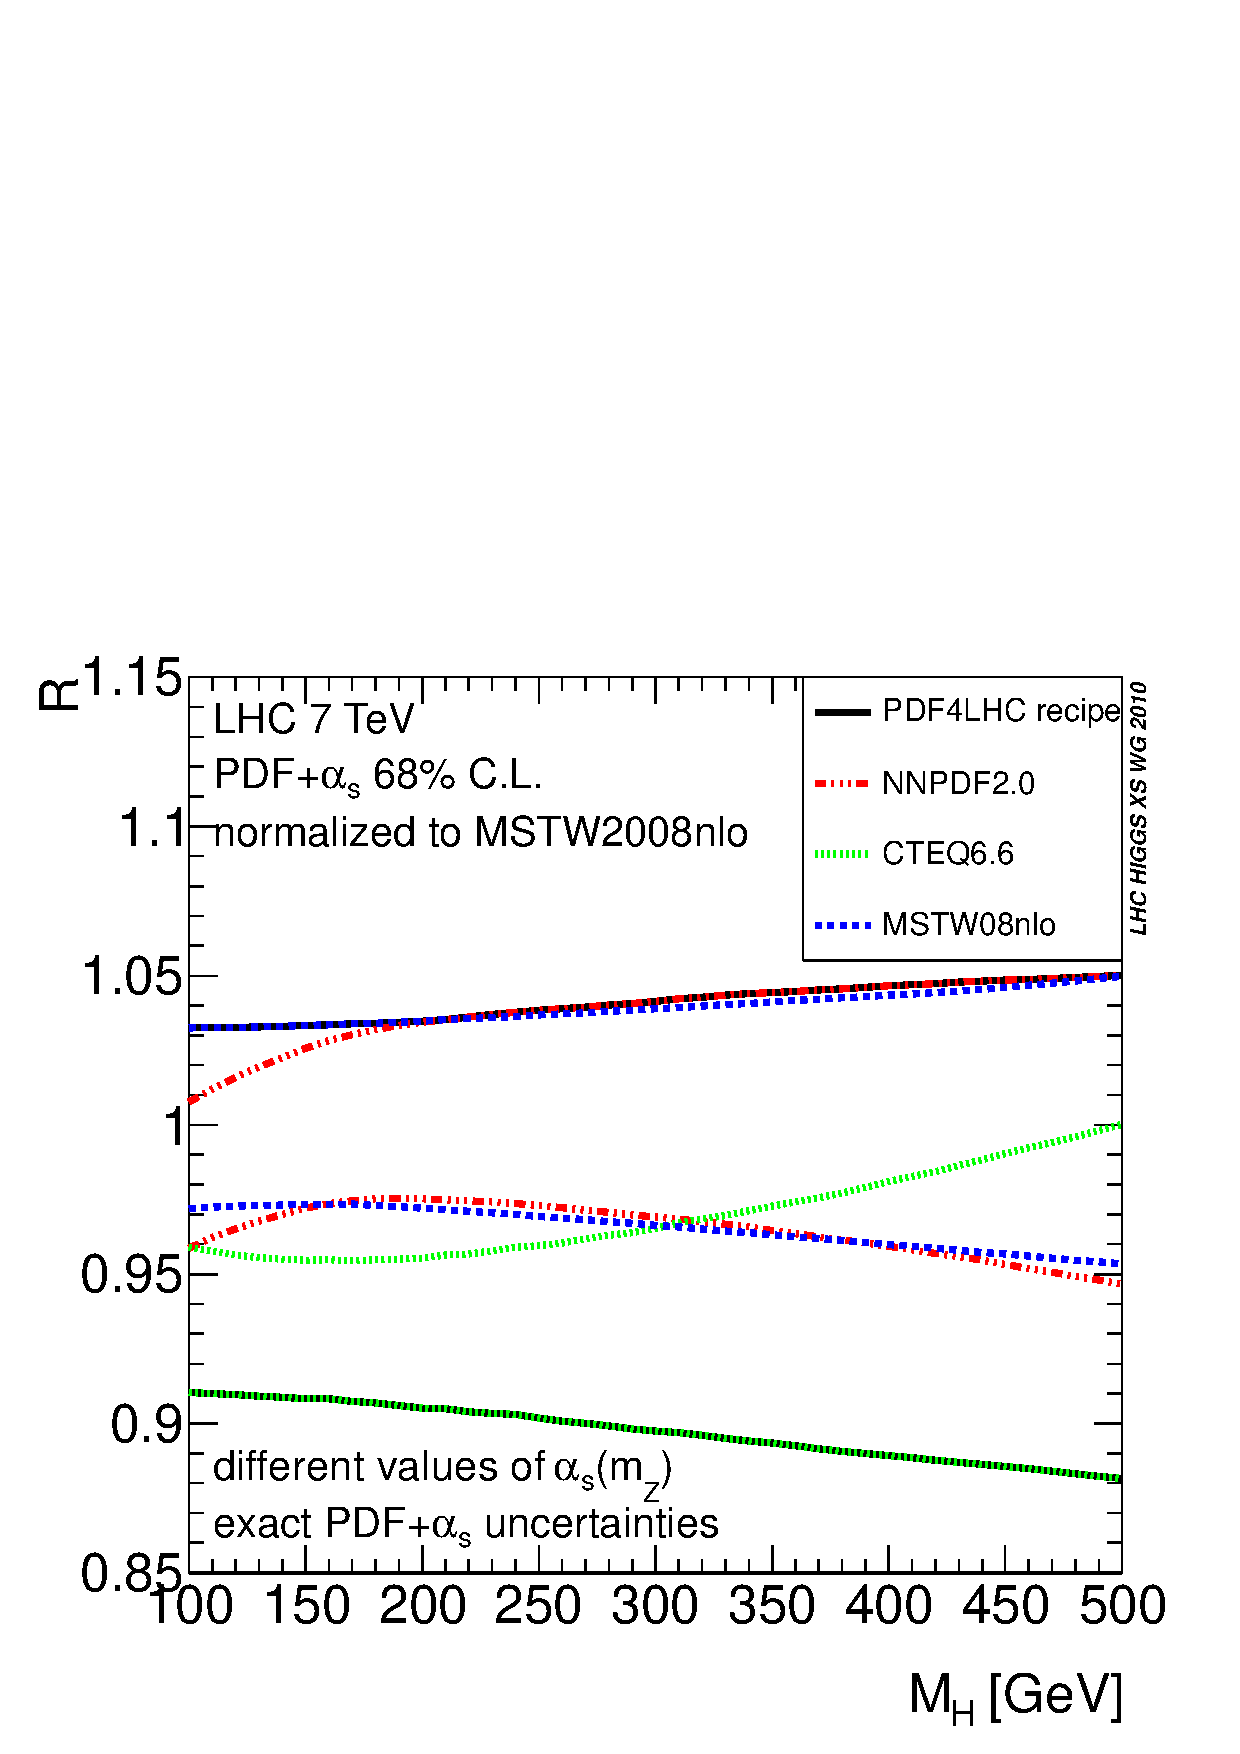
\includegraphics[height=55mm,angle=0]{YRHXS_PDF/YRHXS_PDF_6}
% 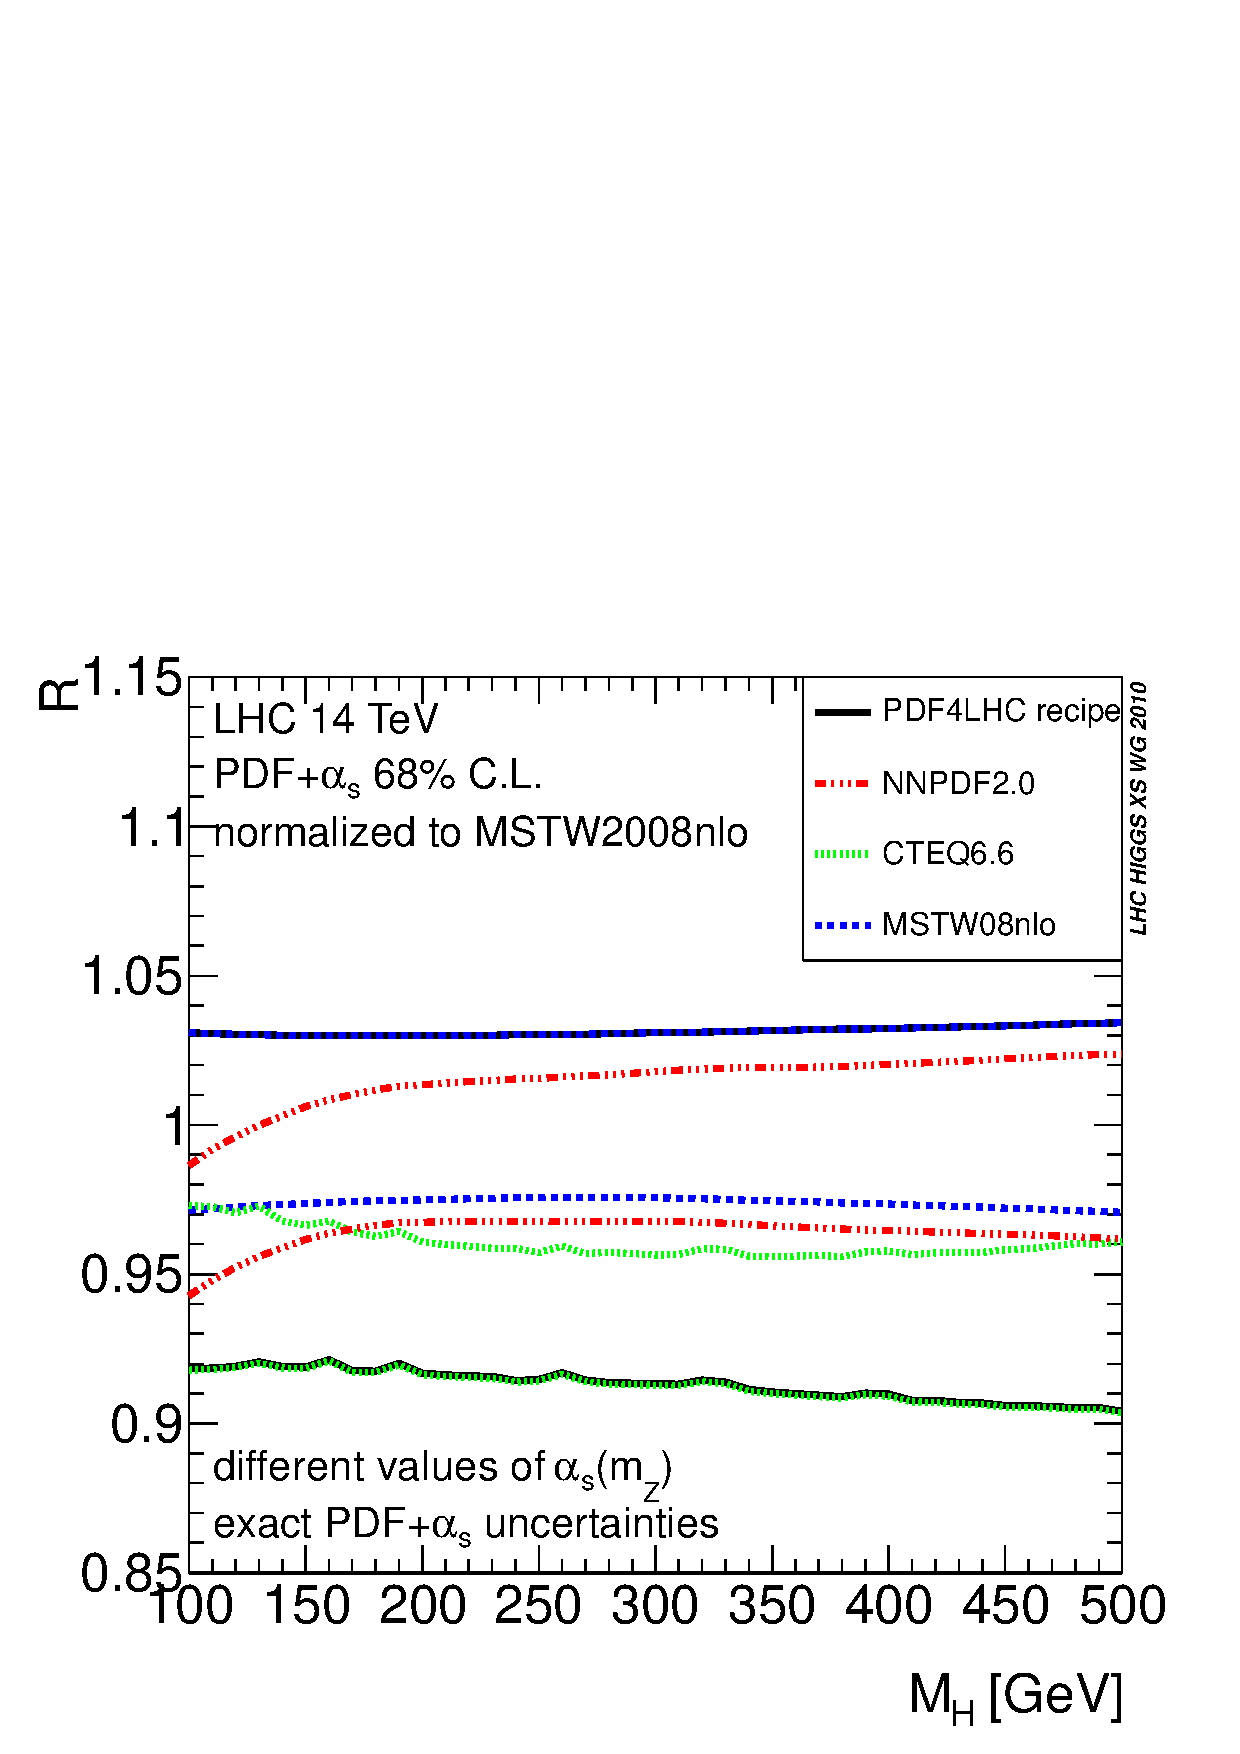
\includegraphics[height=55mm,angle=0]{YRHXS_PDF/YRHXS_PDF_7}
  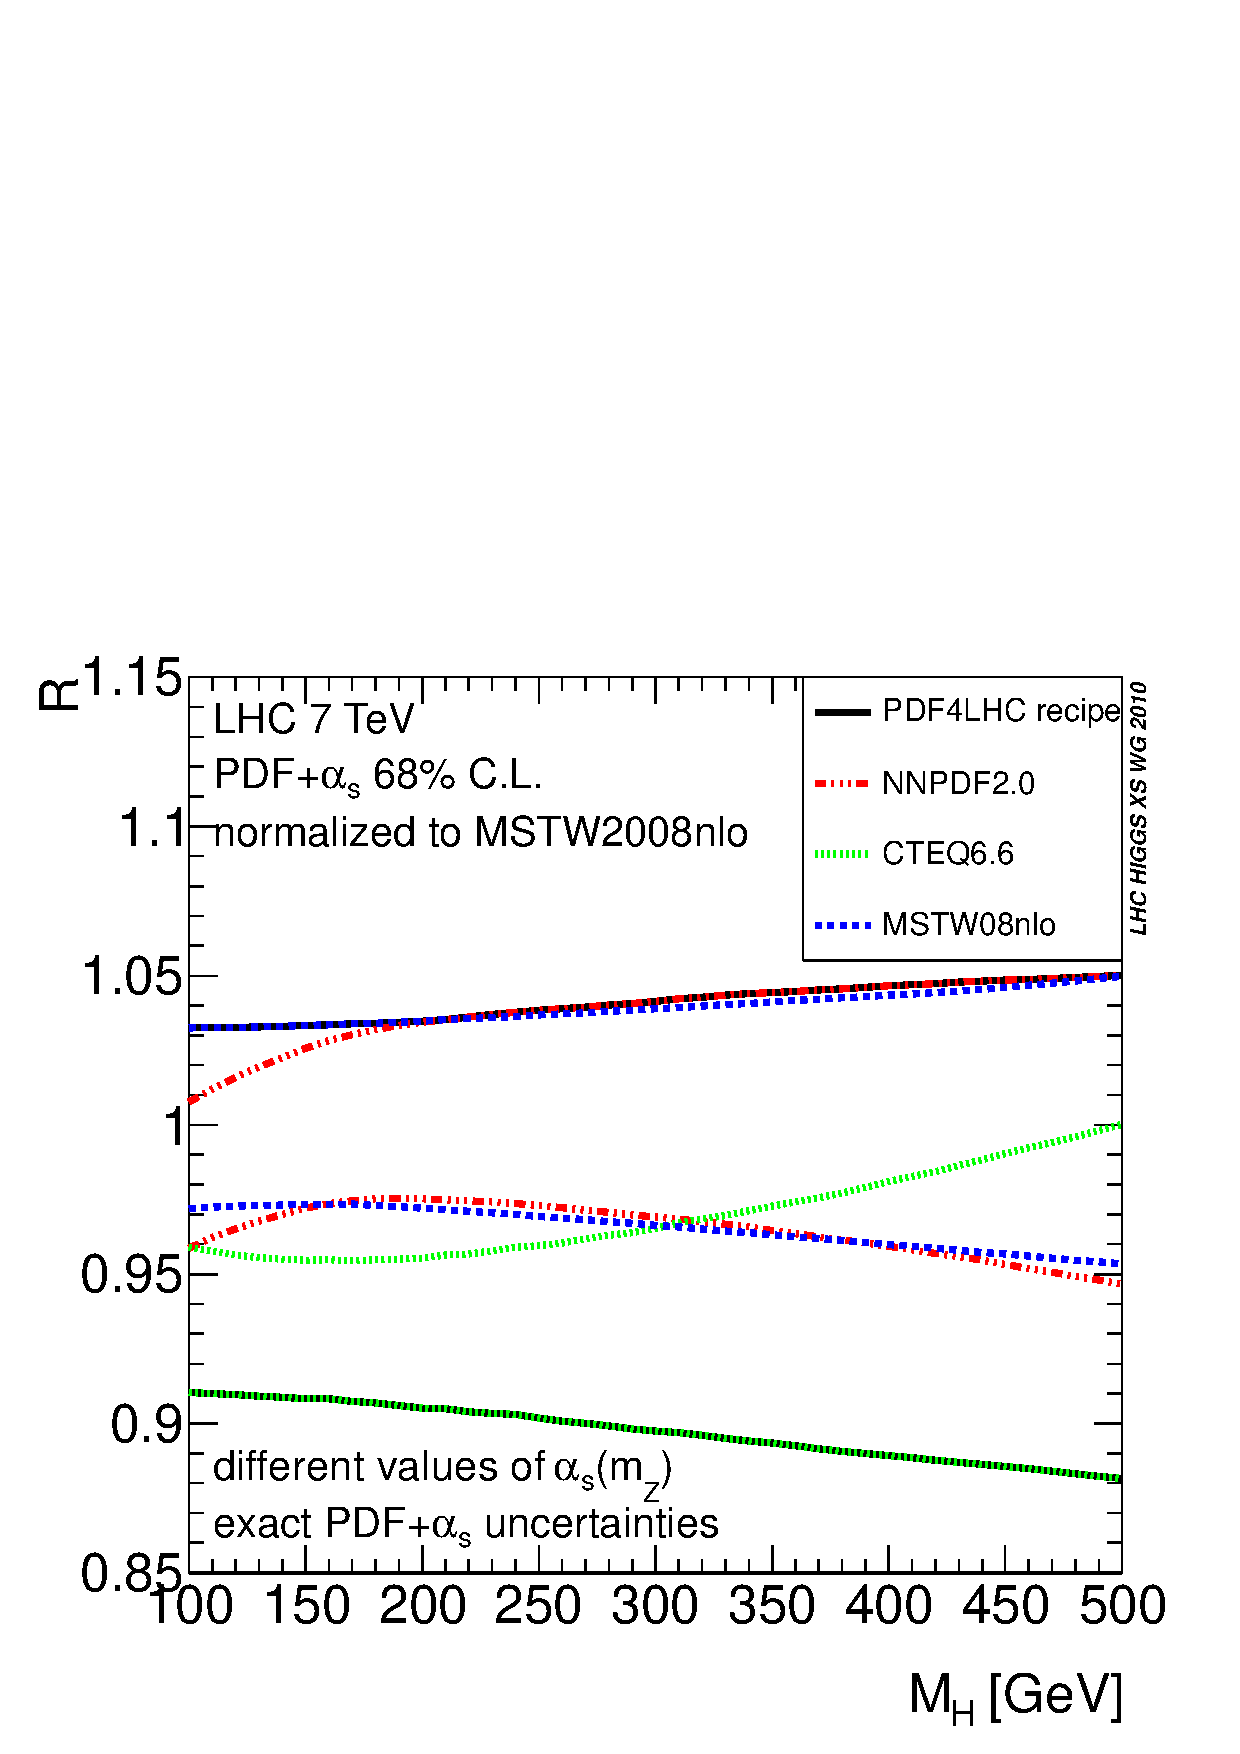
\includegraphics[width=0.48\textwidth]{YRHXS_PDF/YRHXS_PDF_6}
  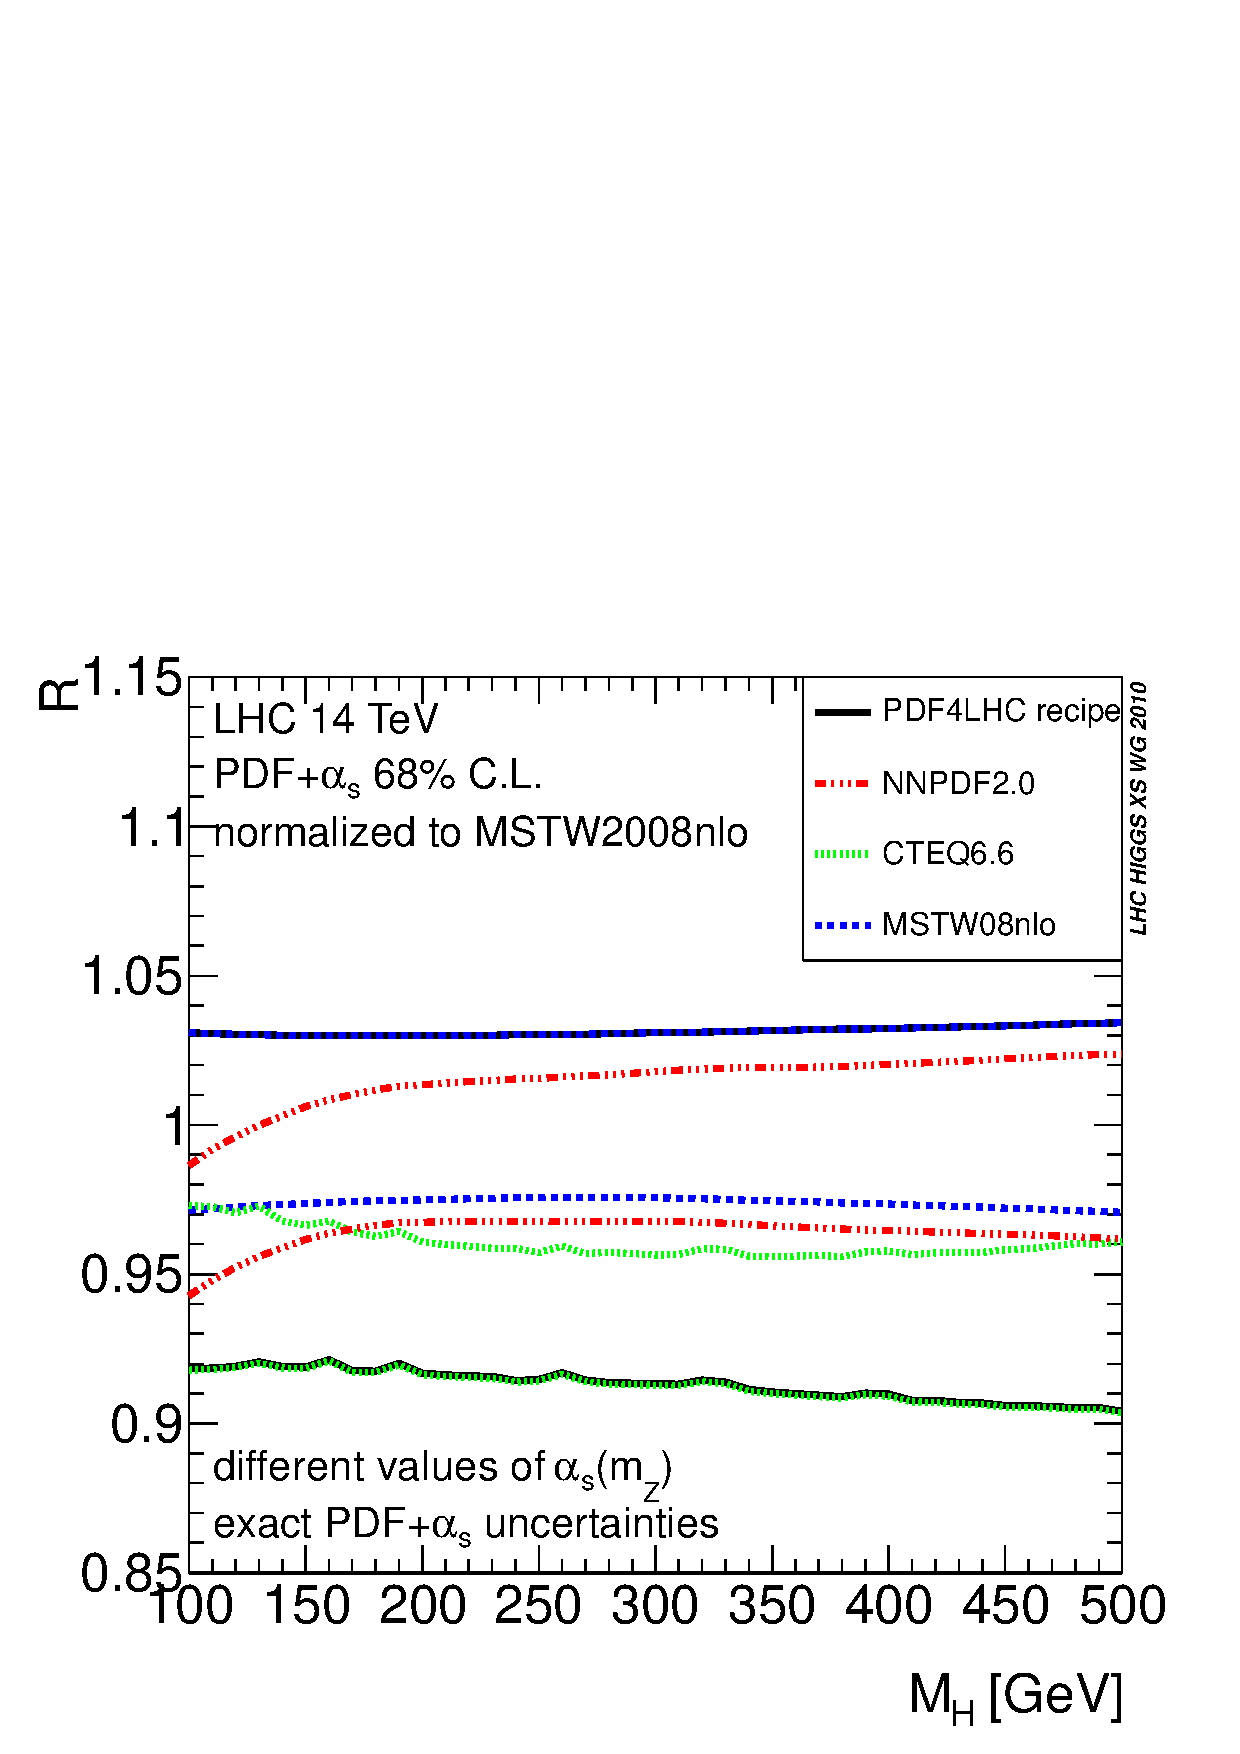
\includegraphics[width=0.48\textwidth]{YRHXS_PDF/YRHXS_PDF_7}
\end{center}
\vspace{-0.6cm}
\caption{Combined PDF+$\alphas$ uncertainty band
for the total Higgs production cross section via gluon fusion,
at NLO,
evaluated according to the PDF4LHC recipe.
The bands are normalized to the central MSTW2008 NLO result.}
\vspace{-0.6cm}
\label{nloenvelope}
\end{figure}

\subsection{The PDF4LHC recommendation}
\label{sec:pdf4lhcreco}

Before we present our recommendation, we would like to highlight the
differences between two use cases: (1) cross sections which have not
yet been measured (such as, for example, Higgs production) and (2)
comparisons to existing cross sections. For the latter, the most
useful comparisons should be to the predictions using individual PDFs
(and their uncertainty bands) discussed above. Such cross sections
have the potential, for example, to provide information useful for
modification of those PDFs. For the former, in particular the 
cross-section predictions in this Report, we would like to provide a
reliable estimate of the true uncertainty, taking into account
possible differences between the central values of predictions using
different PDFs. From the results seen it is clear that this
uncertainty should be larger than that from any single PDF set; however
in order for the probabilistic interpretation of PDF uncertainties to
be preserved, it should not lose all connection to the individual PDF
uncertainties, which would inevitably happen for many processes if the full
spread of all PDFs were used. In order to do this,  
some compromise must be  reached.  


As seen at NLO there is always reasonable agreement
between MSTW, CTEQ, and NNPDF, and potentially more deviation with the other 
sets. In some cases this deviation has at least one potential origin,
 e.g.\ the $\PQt\PAQt$ 
cross section at $7$\UTeV\ at the LHC probes similar PDFs as probed in
 the lower-$\pT$ 
jet production at the Tevatron, which has neither been fit nor validated 
against quantitatively by some groups (preliminary results for ABM may be 
found at \Brefs{Trento,PDF4LHCnov10}). As noted, large deviations 
in predictions between 
existing NNLO sets are similar to those between the same NLO sets.
Discrepancies in MSTW, CTEQ, and NNPDF
do not always have clear origin, or may be a matter of procedure (e.g.\ gluon 
parametrization) which is an ongoing debate between groups. Bearing this in 
mind and having been requested to provide a procedure to give a moderately 
conservative uncertainty, we adopt the following
PDF4LHC recommendation~\cite{PDF4LHCwebpage}. 

\subsubsection{NLO prescription}

At NLO the recommendation is to use (at least) 
predictions from the PDF fits from CTEQ, MSTW, and
NNPDF. These sets all use results from a hadron collider experiment, i.e.,\ the
Tevatron as well as fixed-target experiments and HERA,
and they make available specific sets for a
variety of values of $\alphas$. The PDF versions to be used are: CTEQ6.6,
MSTW2008, and NNPDF2.0. Neither the CTEQ6.6 nor the MSTW2008 
use the new combined very accurate HERA data sets, whereas NNPDF2.0 does
use this data (the CT10~\cite{Lai:2010vv}   update of 
the CTEQ PDFs does include them and future updates of MSTW~\cite{Thorne:2010kj} will
as well). It is to be noted 
that CTEQ6.6 and MSTW2008 are the PDF versions most commonly used by the LHC
experiments currently, hence it is these
versions that are suggested in the recommendation.
 The NNPDF2.0 set does not use a general-mass variable flavour
number scheme (the NNPDF2.1 PDF set, which does use a general-mass
variable flavour number scheme is currently being
finalized~\cite{Rojo:2010gv}), but the
alternative method which NNPDF use for determining PDF uncertainties
provides important independent information.  
Other PDF sets, GJR08, ABKM09, and HERAPDF1.0 are useful for more 
conservative or extensive evaluations of the uncertainty.  
For example a study of the 
theoretical uncertainties related to the charm-mass treatment is possible 
using HERAPDF1.0 and ABKM. 

The  $\alphas$ uncertainties can be evaluated by
taking a range of $\pm 0.0012$ for $68\%$~CL (or $\pm 0.002$ for $90\%$~CL) from the preferred central value for CTEQ and NNPDF. The total
PDF+$\alphas$ uncertainty can then be evaluated by adding the
variations in PDFs due to $\alphas$ uncertainty in quadrature with
the fixed $\alphas$ PDF uncertainty (shown~\cite{Lai:2010nw} 
to correctly incorporate
correlations in the quadratic error approximation) or, for NNPDF,
more efficiently taking a gaussian distribution of PDF replicas
corresponding to different values of $\alphas$. 
For MSTW the PDF+$\alphas$ uncertainties should be evaluated using
their prescription which better accounts for correlations between the
PDF and $\alphas$ uncertainties when using the MSTW dynamical
tolerance procedure for uncertainties. Adding the $\alphas$
uncertainty in quadrature for MSTW can be used as a simplification but
generally gives slightly smaller uncertainties.  

So the prescription for NLO is as follows:


\begin{itemize}

\item For the  calculation of uncertainties at the LHC, use  the
  envelope provided by the central values and PDF+$\alphas$ errors
  from the MSTW08, CTEQ6.6, and NNPDF2.0 PDFs, using each group's
  prescriptions for combining the two types of errors. We propose this
  definition of an envelope because the deviations between the
  predictions can sometimes be  as large as  their uncertainties. 
  As a central value, use the midpoint of this
  envelope. We follow the PDF4LHC prescription and
  recommend that a $68\%$~CL uncertainty envelope be
  calculated and the $\alphas$ variation suggested is consistent with
  this. Note that the CTEQ6.6 set has uncertainties and $\alphas$
  variations provided only at $90\%$~CL and thus their uncertainties
  should be reduced by a factor of $1.645$ for $68\%$~CL. Within the
  quadratic approximation, this procedure is exact.  


\end{itemize}



\subsubsection{NNLO prescription}

For estimating uncertainties in cross section at NNLO, the 
recommendation is to use for base predictions 
the only NNLO set which currently includes a wide variety of hadron 
collider data sets, i.e.,\ MSTW2008. There seems to be
no reason to expect that the spread in predictions of the sets used in the 
NLO prescription, i.e.,\ MSTW, CTEQ, and NNPDF,  will diminish significantly 
at NNLO compared to NLO, where this spread was somewhat larger than the 
uncertainty from each single group. 
Hence, at NNLO the uncertainty obtained from MSTW alone should be expanded 
to some degree. It seems appropriate to do this by multiplying the MSTW 
uncertainty at NNLO by the factor obtained by dividing the full uncertainty 
obtained from the envelope of MSTW, CTEQ, and NNPDF results at NLO by the 
MSTW uncertainty at NLO. In all cases the $\alphas$ uncertainty should be 
included. We note that in several cases so far examined, for the LHC running at 
$7$\UTeV\ centre-of-mass energy, this factor of the envelope divided by the 
MSTW uncertainty is approximately constant, and 
quite close to $2$ for Higgs production as shown below: 
this constant factor can be used as a 
short-hand prescription. 

Since there are NNLO PDFs obtained from fits including fewer data sets by 
the ABKM, JR, and HERAPDF groups, these should ideally be compared with the 
above procedure, bearing in mind that it is possible there will be kinematic 
regions where the absence of data, or other reasons -- e.g.\ in the JR case 
a theoretical 
constraint is imposed on the input by the choice of assuming the form
Eq.~(\ref{pdfparm}) of PDFs at a very low, arguably non-perturbative,
starting scale (though data are fit only at higher scales) -- may lead to PDFs and predictions differing 
significantly from the central value and the extent of the uncertainty band.


So the prescription at NNLO is:

\begin{itemize}

\item As a central value, use the MSTW08 prediction. As an uncertainty, take the same percentage uncertainty on this NNLO prediction as found using the  NLO uncertainty prescription given above.

\end{itemize}


\subsubsection{Application to Higgs production via gluon fusion}
\label{sec:pdf4lchiggs}

%The total hadronic cross section
%for the inclusive production of a Higgs boson via gluon fusion
%can be written 
%\be
%\sigma(h_1 h_2\to H+X)
%=
%\sum_{a,b}\int_0^1 dx_1 dx_2~
%f_{a,h_1}(x_1,\mu_F^2) f_{b,h_2}(x_2,\mu_F^2)
%~
%\int_0^1 dz~
%\delta\left(
%z-\frac{\tau_H}{x_1 x_2}
%\right)
%\hat\sigma_{ab}(z)
%\ee

%The accurate evaluation of
%the partonic cross section $\hat \sigma_{ab}$
%is the most important step to obtain an accurate prediction of
%the central value of the total hadronic cross section.
%In fact the latter receives large contributions from NLO- and NNLO-QCD
%corrections, but also from the soft gluon resummation, from leading
%NNNLO-QCD terms and from NLO-EW corrections.
%Finite top mass corrections at NNLO-QCD have been studied and turn out
%to be small.
%For the sake of simplicity but still in full generality,
%the evaluation of the size of the combined PDF+$\alphas$ uncertainty
%can be obtained by considering only exact NLO-QCD and NNLO-QCD corrections
%in the infinite top mass limit.

\begin{figure}
  \begin{center}
%    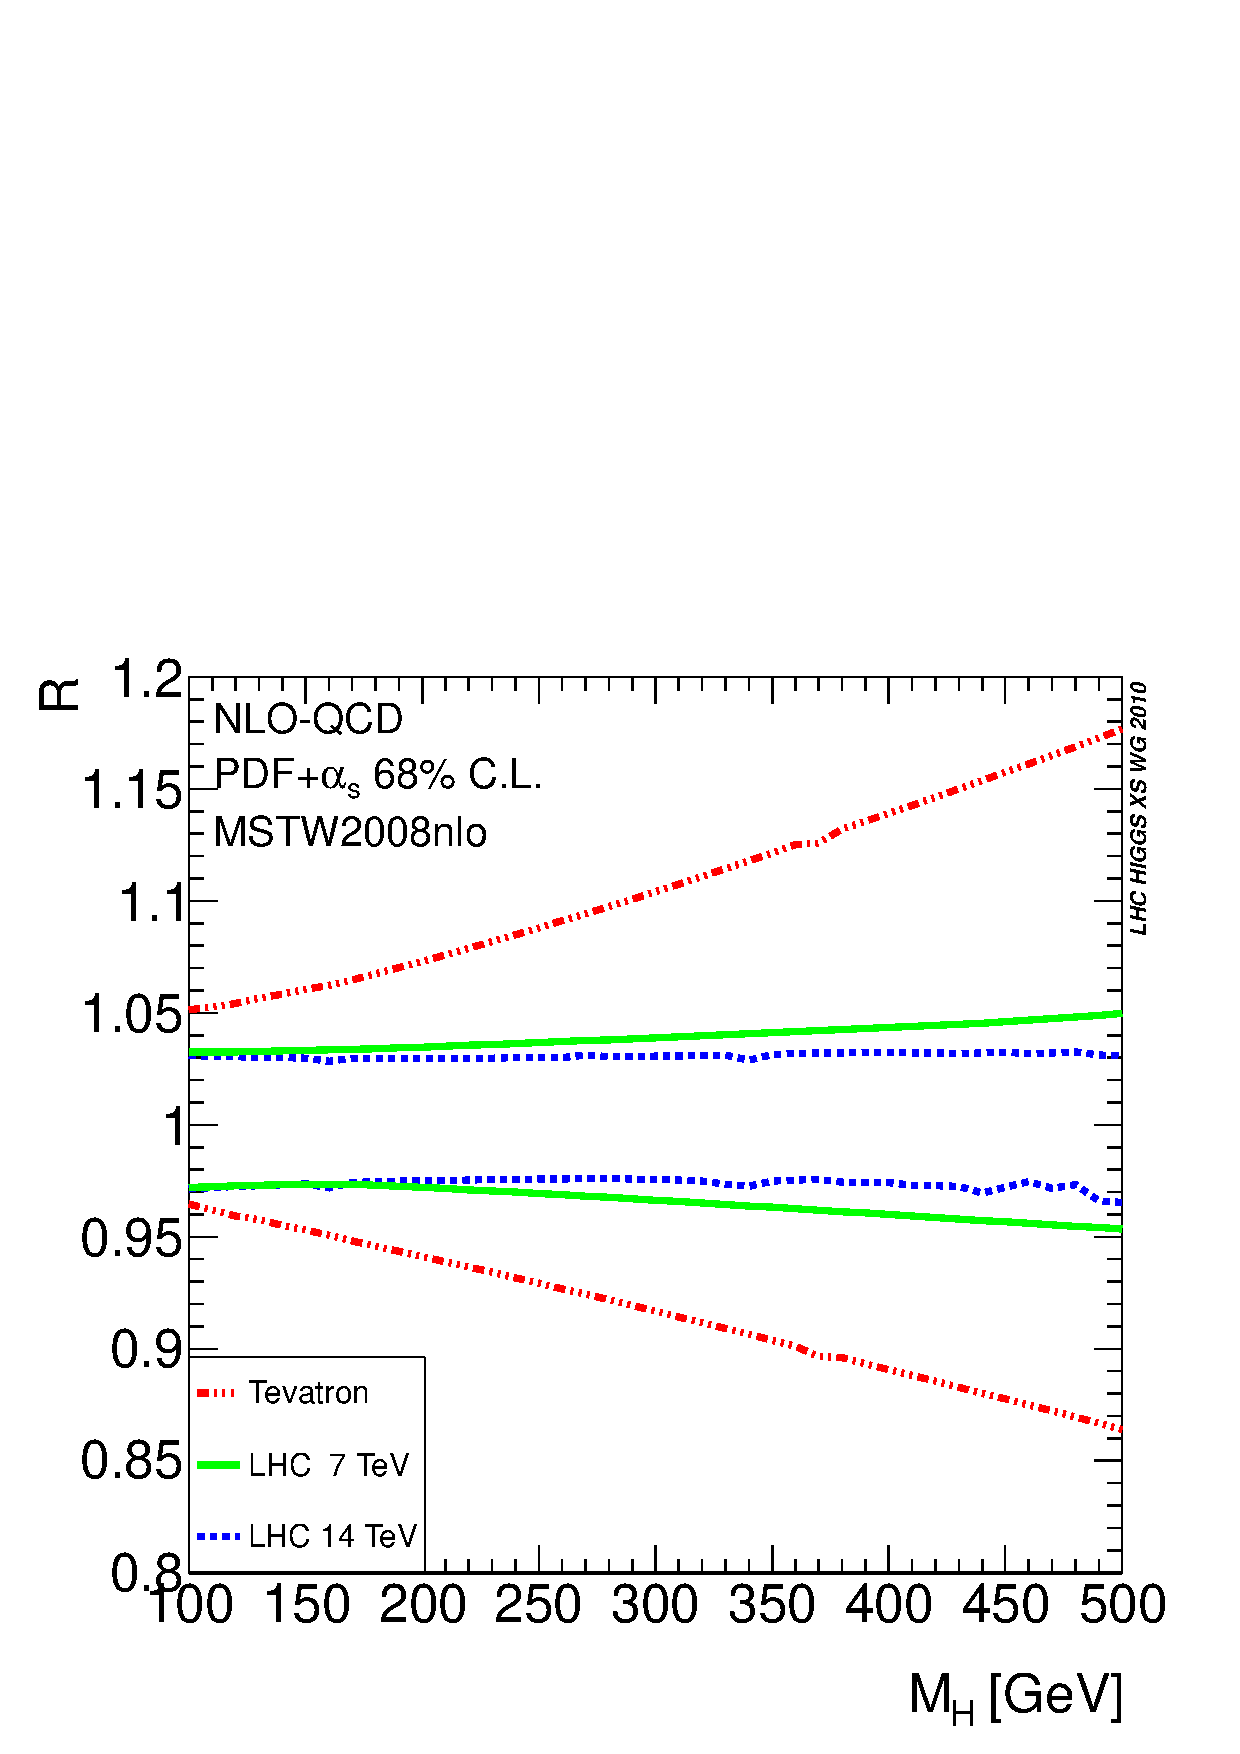
\includegraphics[height=55mm,angle=0]{YRHXS_PDF/YRHXS_PDF_8}
%    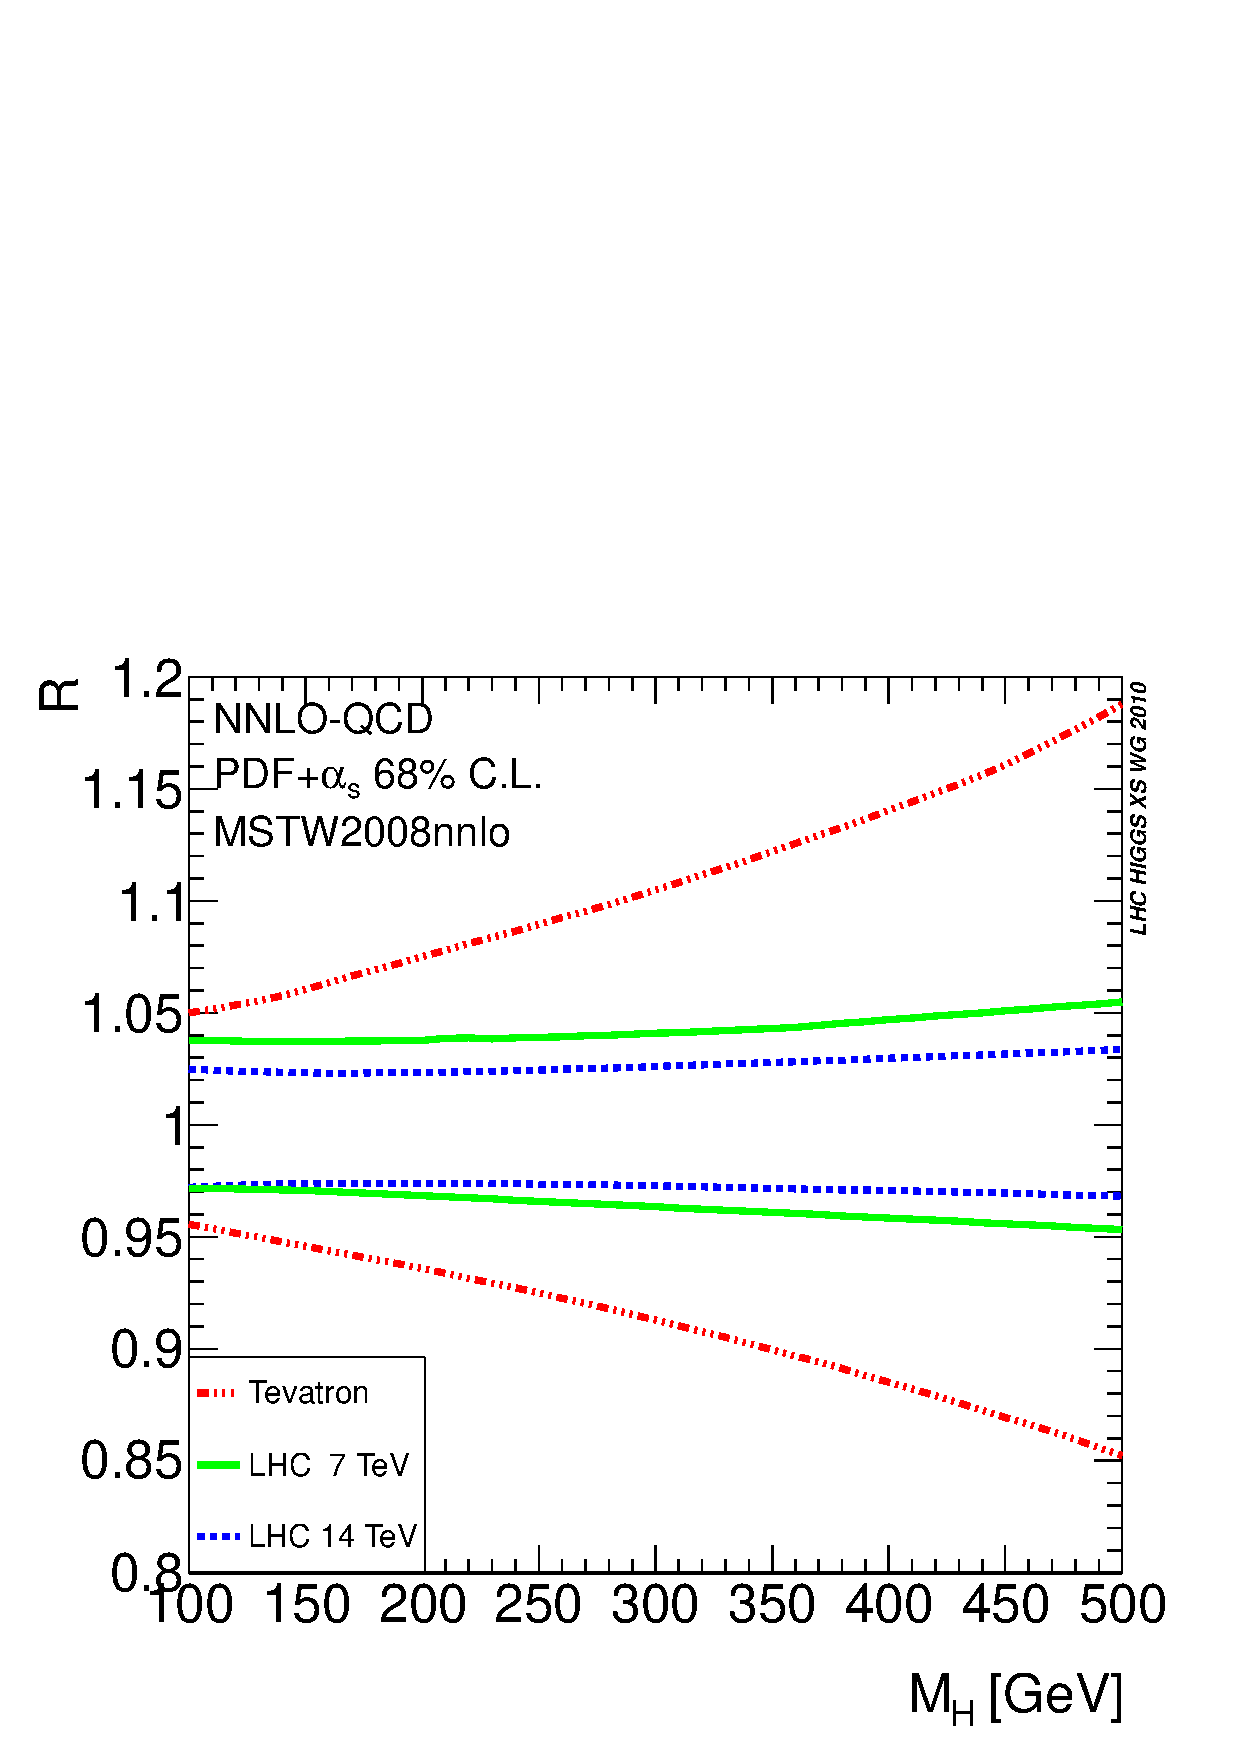
\includegraphics[height=55mm,angle=0]{YRHXS_PDF/YRHXS_PDF_9}\\%[5mm]
    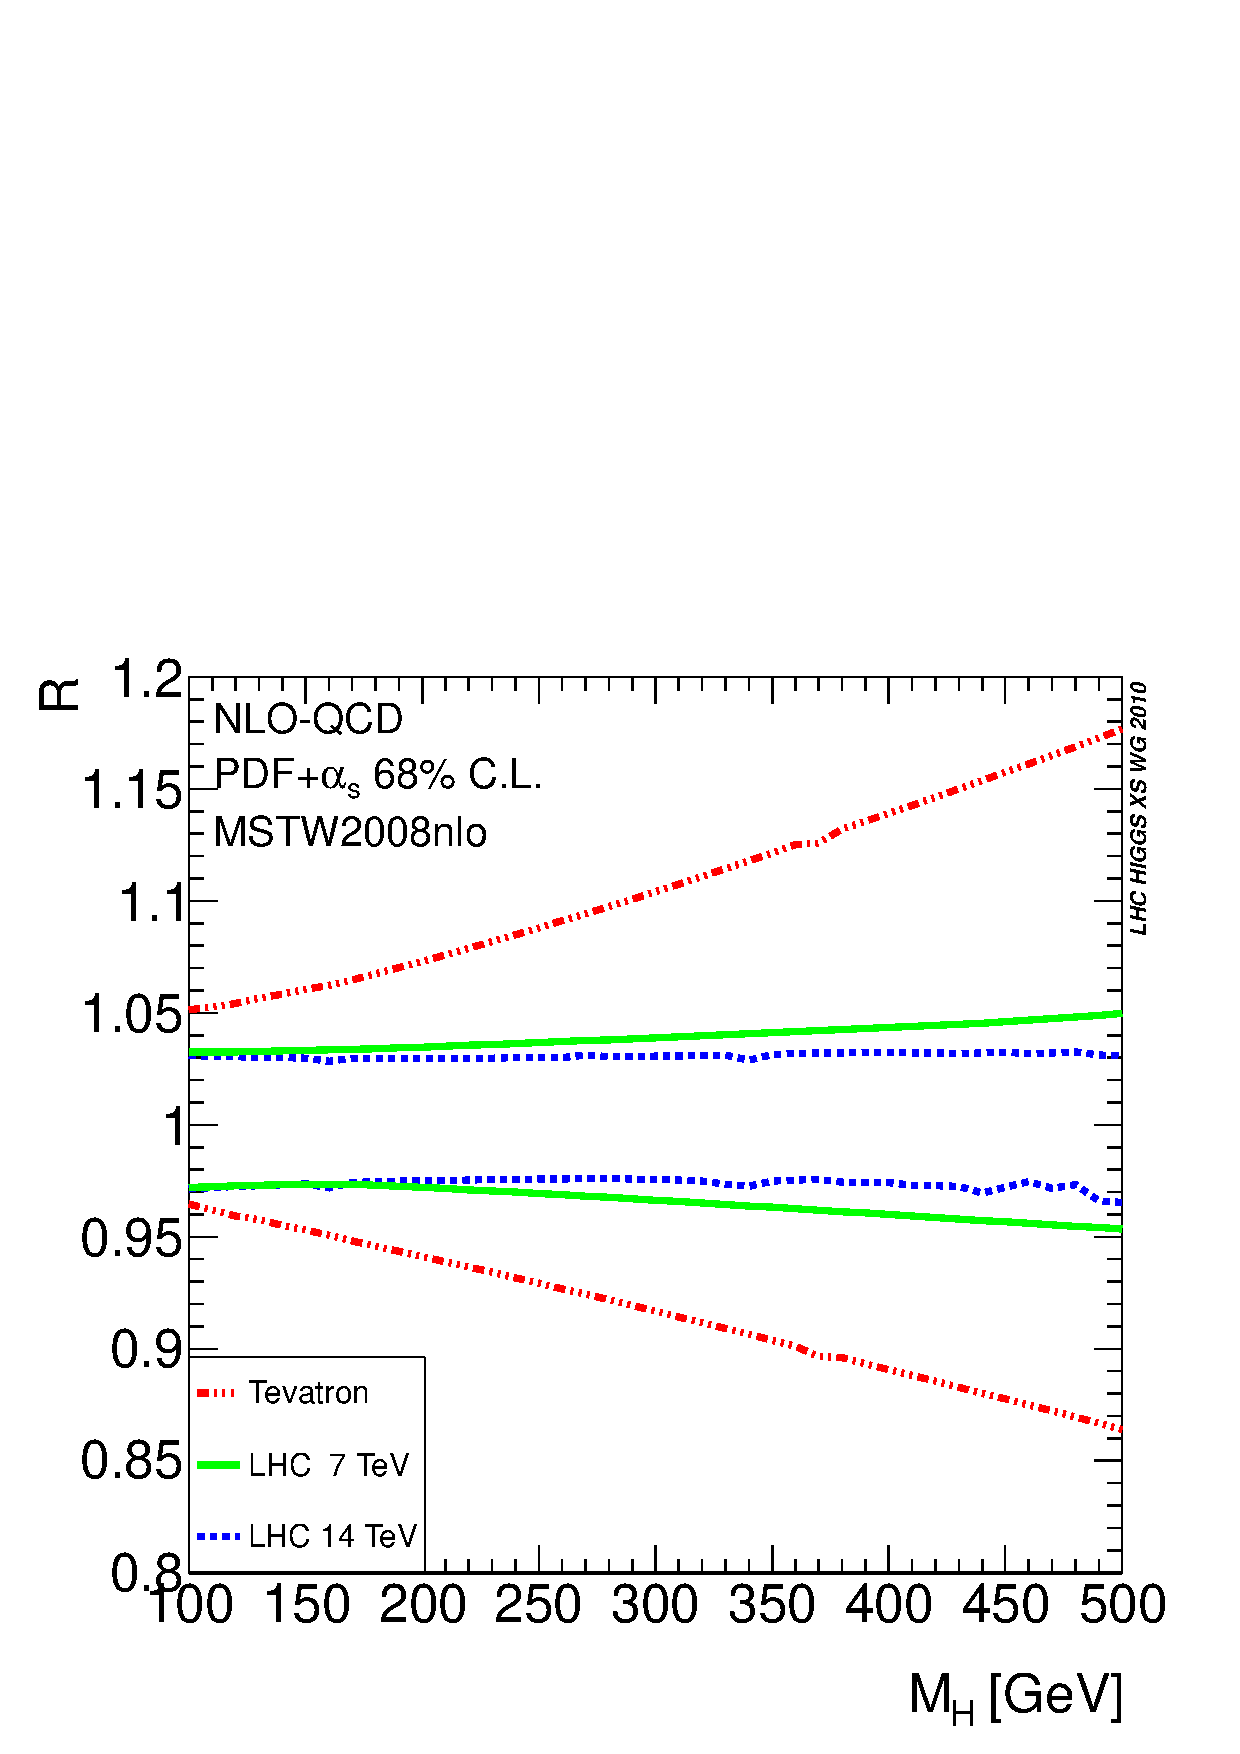
\includegraphics[width=0.48\textwidth]{YRHXS_PDF/YRHXS_PDF_8}
    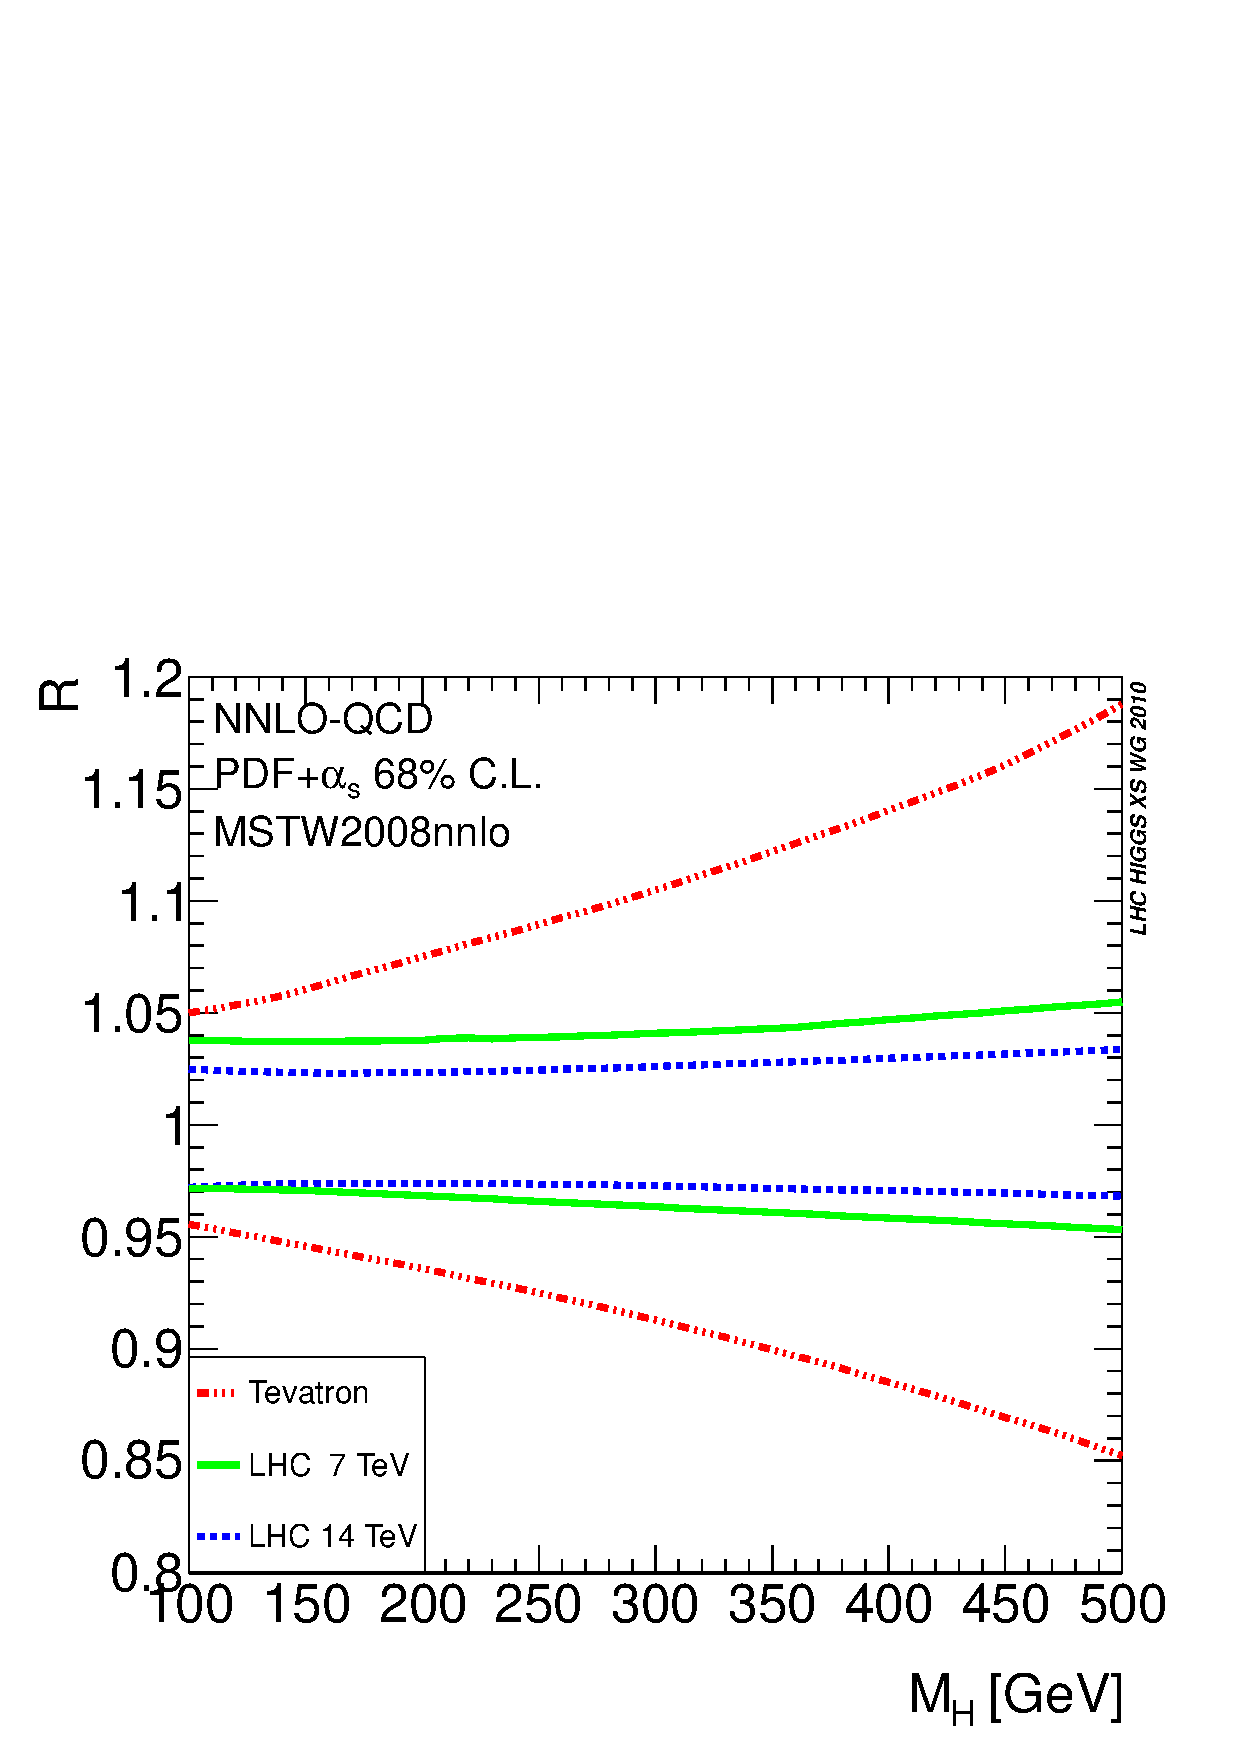
\includegraphics[width=0.48\textwidth]{YRHXS_PDF/YRHXS_PDF_9}\\%[5mm]
    %\vspace{-0.5cm}
%    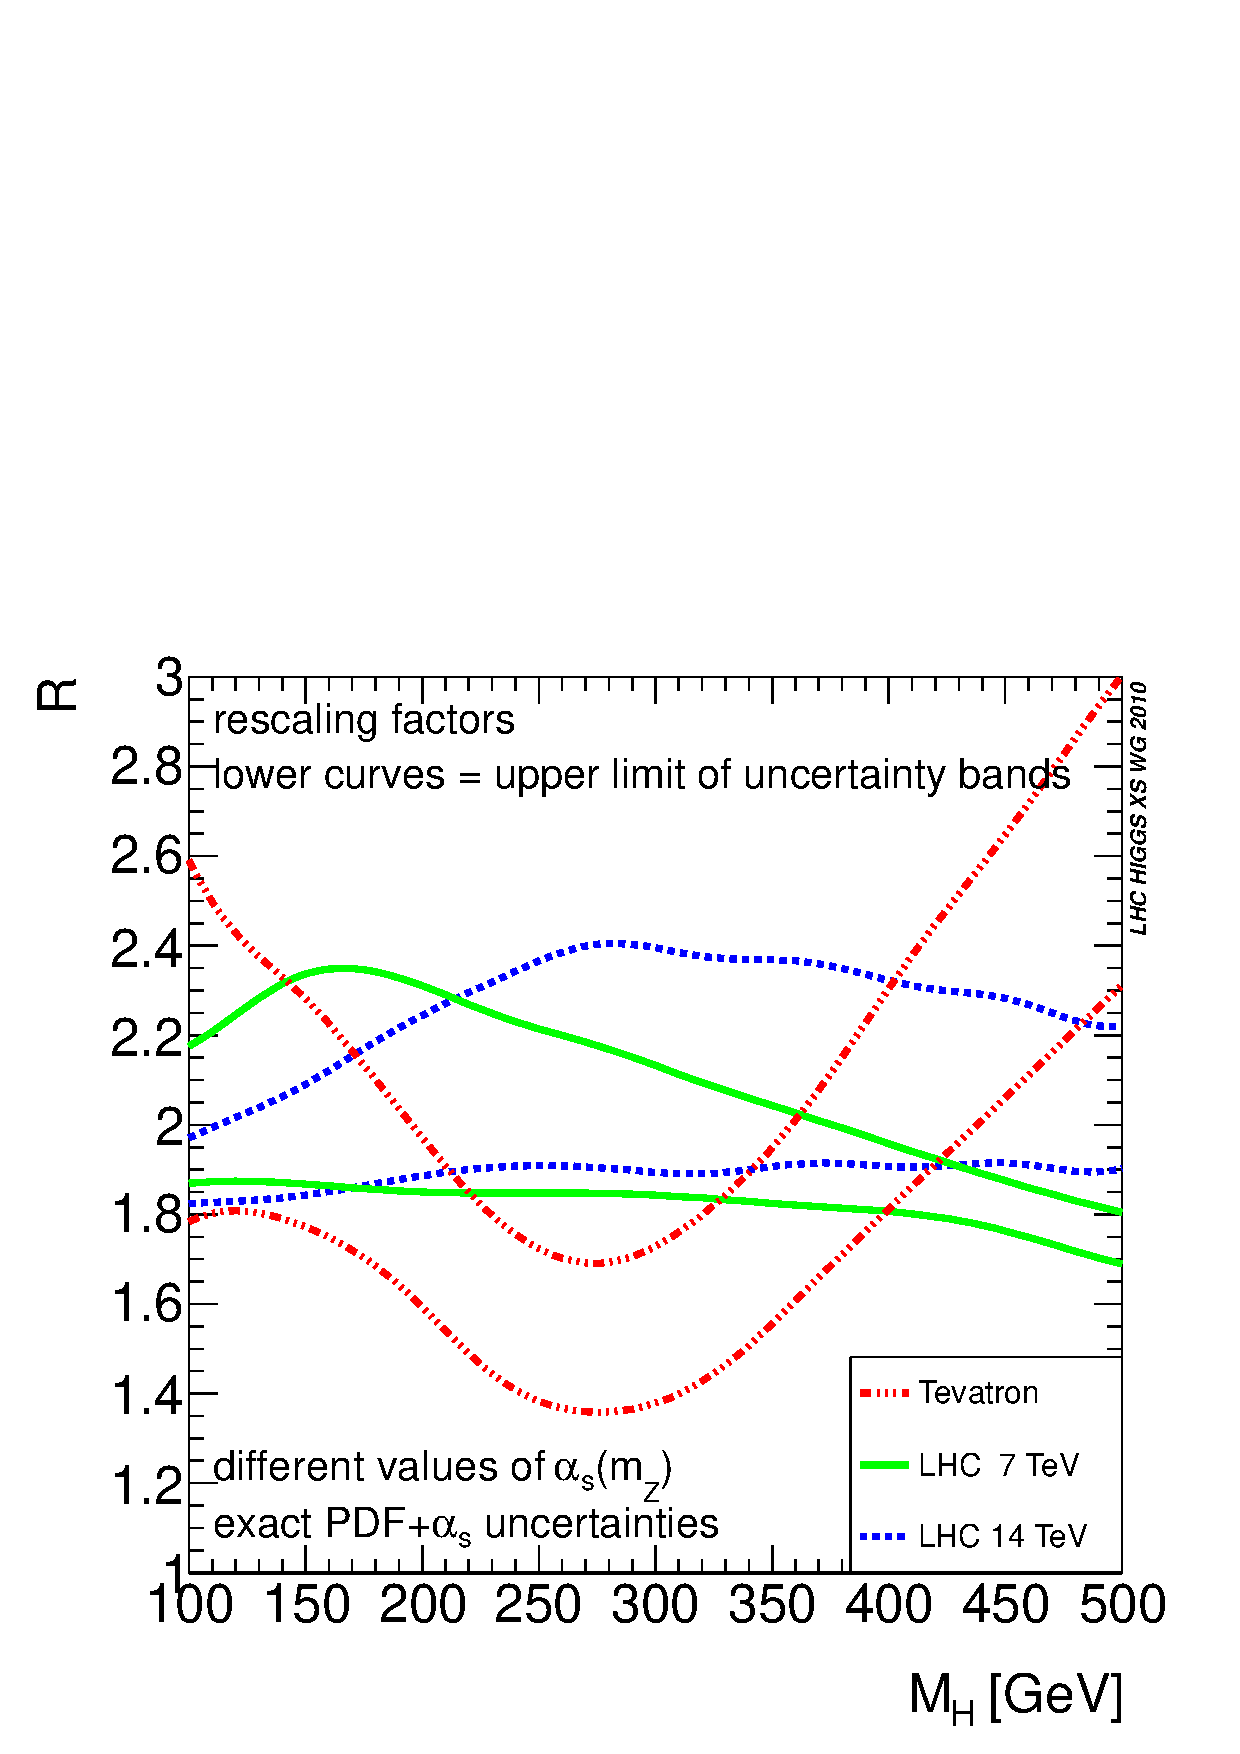
\includegraphics[height=55mm,angle=0]{YRHXS_PDF/YRHXS_PDF_10}
%    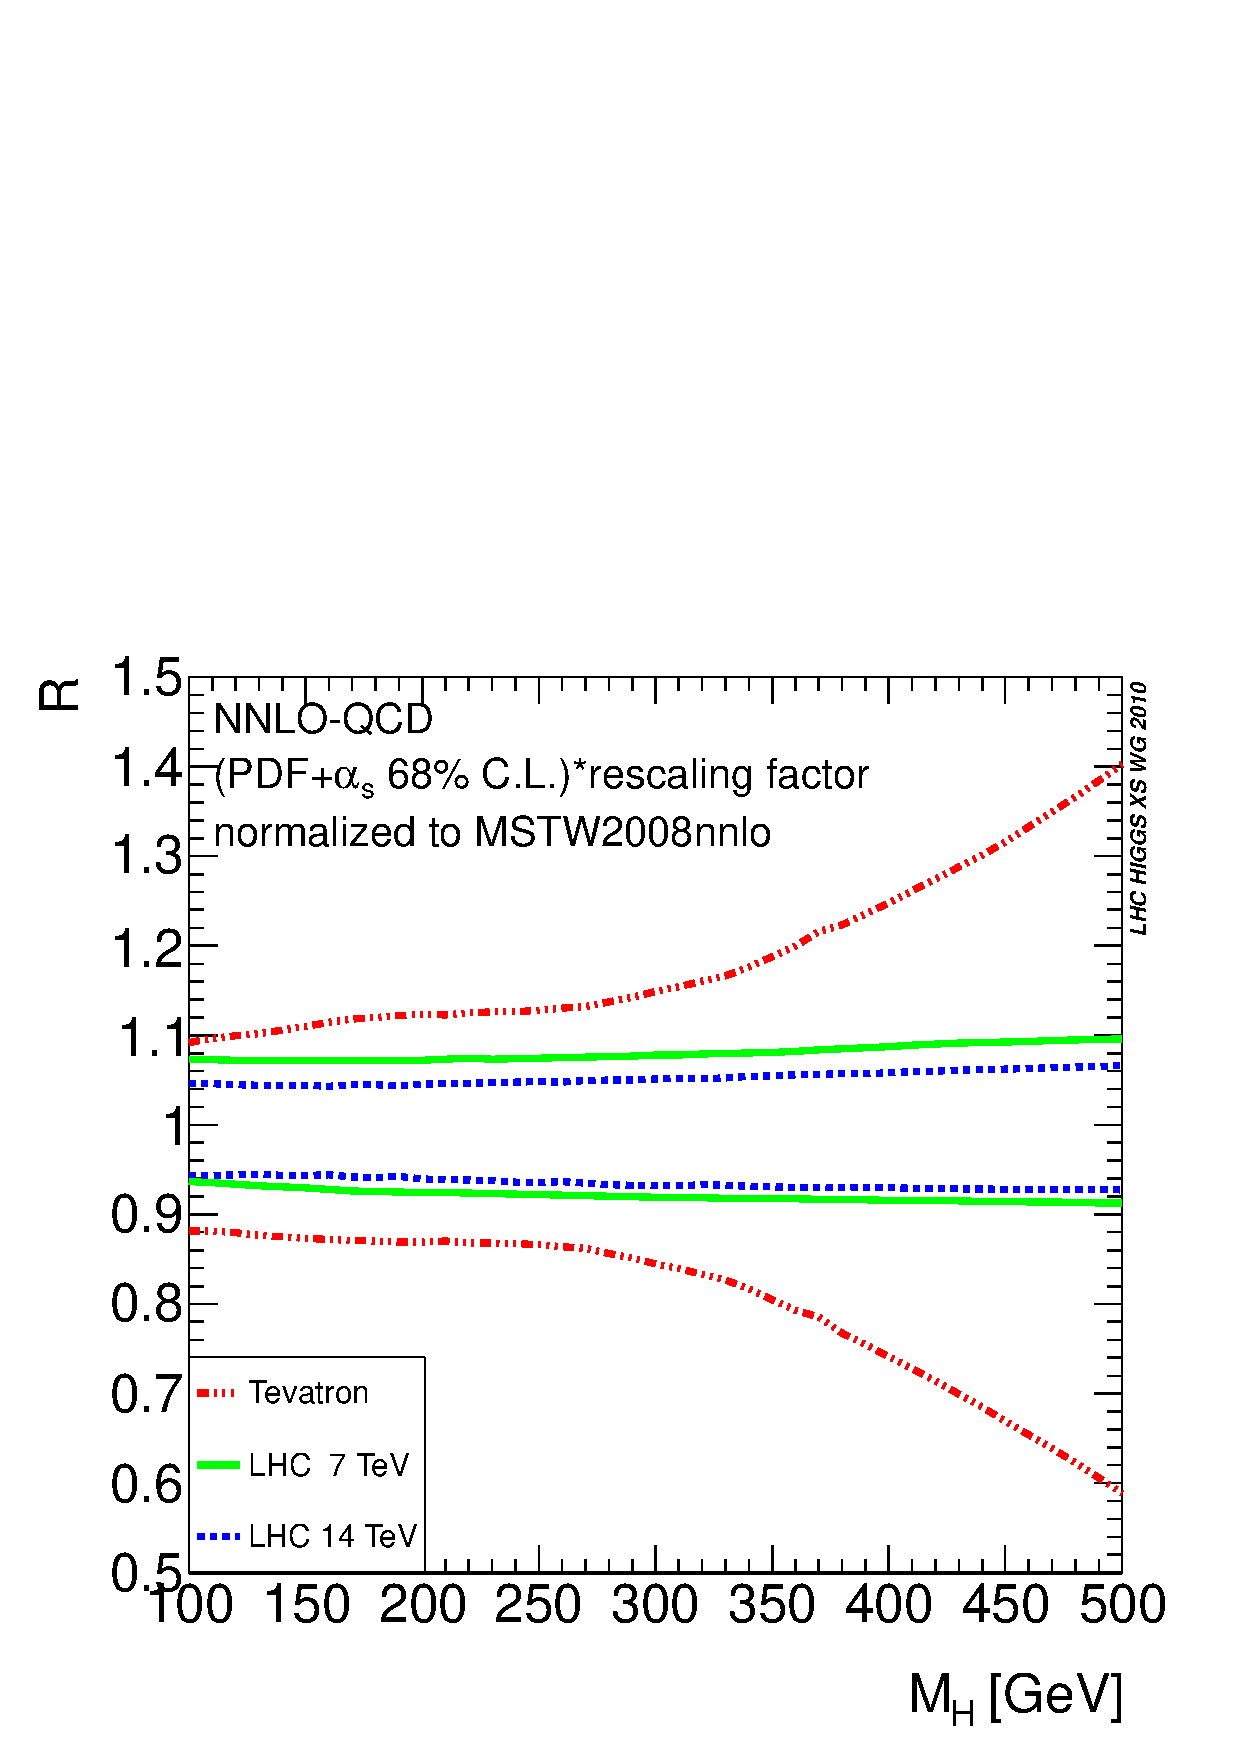
\includegraphics[height=55mm,angle=0]{YRHXS_PDF/YRHXS_PDF_11}
    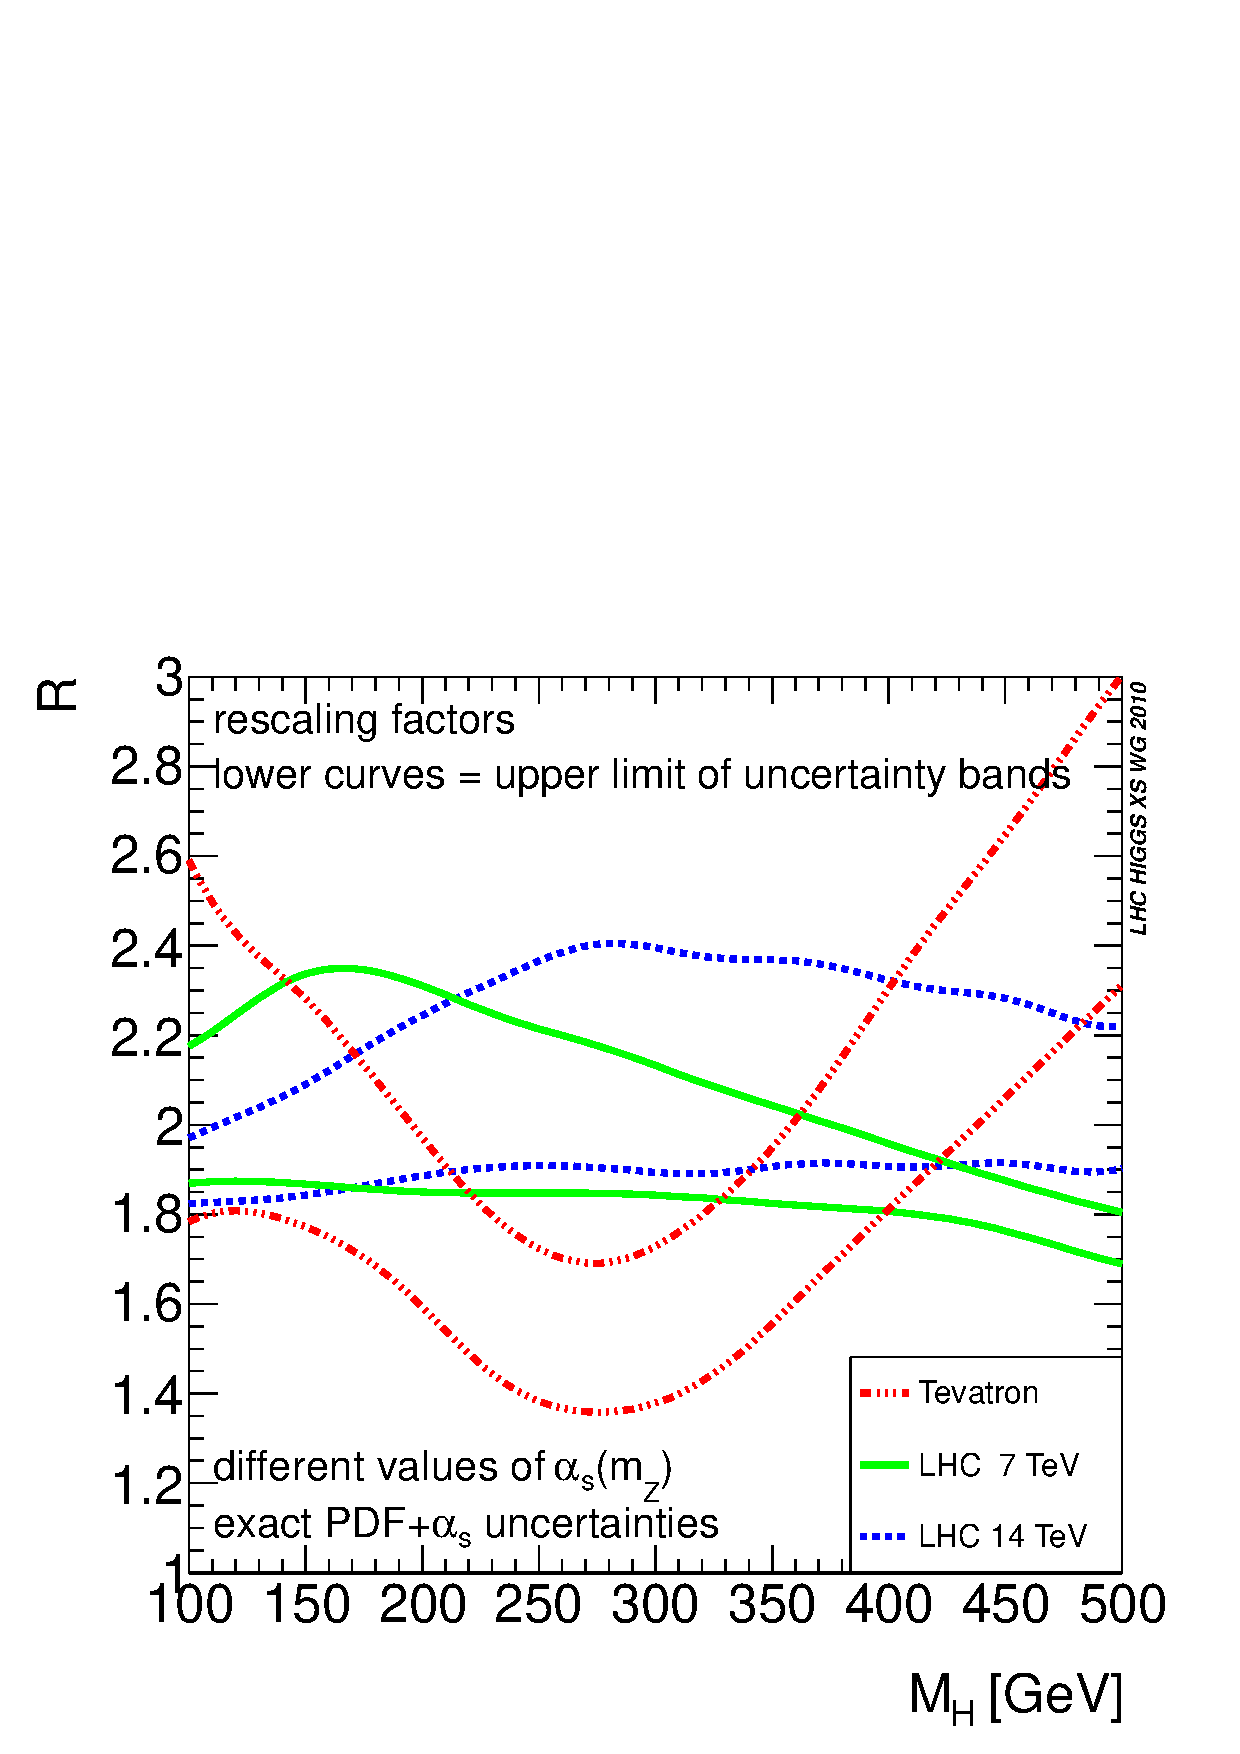
\includegraphics[width=0.48\textwidth]{YRHXS_PDF/YRHXS_PDF_10}
    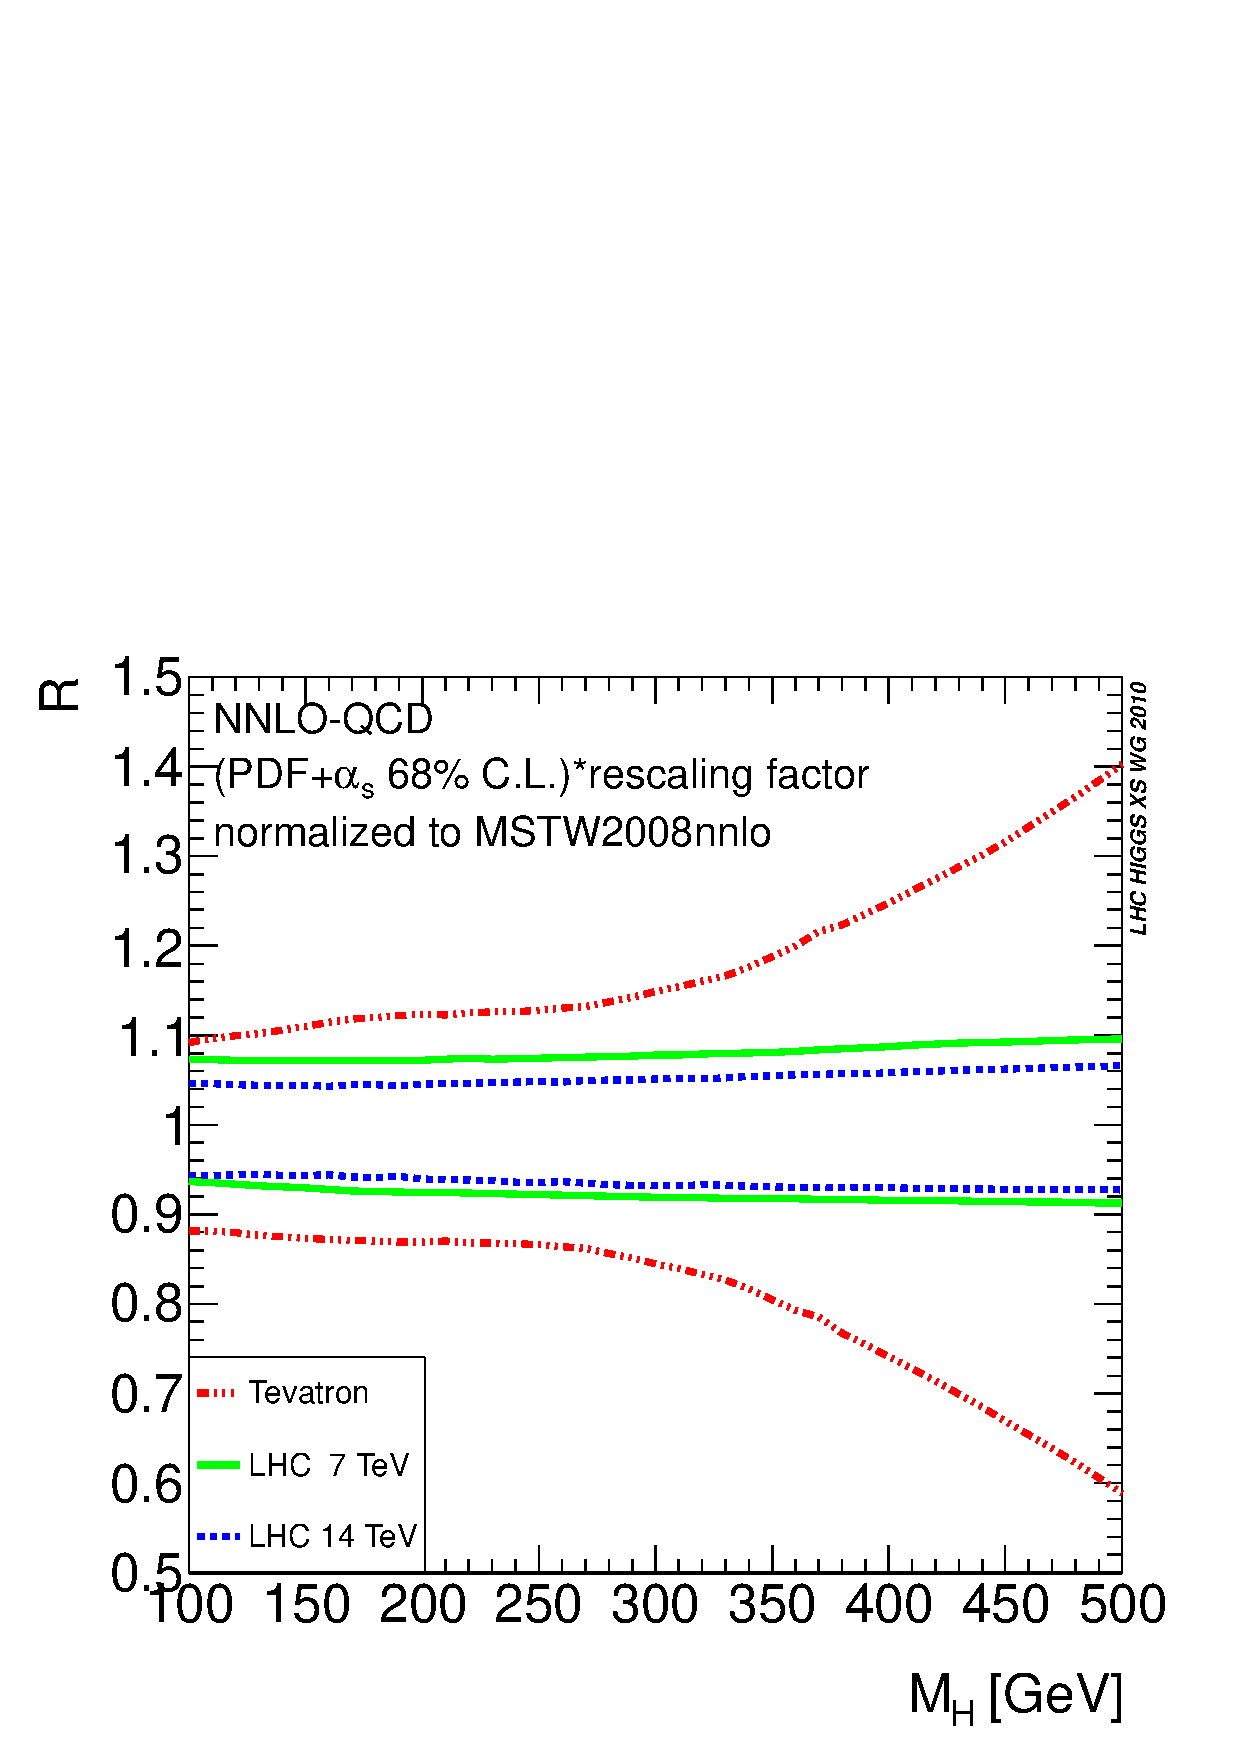
\includegraphics[width=0.48\textwidth]{YRHXS_PDF/YRHXS_PDF_11}    
  \end{center}
  \vspace{-0.8cm}
\caption{
Top: Combined relative PDF+$\alphas$ uncertainty band
for the total  Higgs cross section from gluon fusion,
at NLO (left) and at NNLO (right) obtained using MSTW2008.
 Bottom:  rescaling factor for the NNLO uncertainty (left),
obtained as  the ratio of the percentage
  width of the NLO envelope with respect to its mid point
  to the percentage uncertainty of the MSTW2008 NLO band, and final
  NNLO uncertainty band obtained applying the rescaling to the MSTW08
  NNLO result (right).
%The rescaling factor has to be applied to the MSTW2008nnlo PDF+$\alphas$
%band, to obtain an estimate of the NNLO-QCD envelope.
}
\vspace{-0.5cm}
\label{nlonnlo}
\end{figure}
In accordance with the recommendation, we have considered the 
CTEQ6.6~\cite{Nadolsky:2008zw}, 
MSTW2008~\cite{Martin:2009iq, Martin:2009bu}, and
NNPDF2.0~\cite{Ball:2010de} PDF sets. Combined PDF+$\alphas$ uncertainties
for each of the three global sets are computed as discussed in
Sections~\ref{sec:pdfdet1} and~\ref{sec:pdfdet2} (more details are 
in \Bref{Demartin:2010er}). Computations have been performed 
using the code described in
\Brefs{Bonciani:2007ex, Aglietti:2006tp, Aglietti:2004nj, Aglietti:2004ki, Degrassi:2005mc, Degrassi:2004mx}, 
improved with the NNLO corrections~\cite{Harlander:2000mg, Catani:2001ic, Harlander:2001is, Harlander:2002wh, Anastasiou:2002yz, Ravindran:2003um}.


In order to obtain a meaningful comparison between
different PDF sets it is crucial to adopt the same
uncertainty range for the value of $\alphas$. Here we
assume the  same  range as 
for the PDF4LHC benchmarks of \Bref{PDF4LHCwebpage} 
namely
\beq
\delta^{(90)}\alphas=0.002 \quad\mbox{at}\quad 90\%~{\rm CL},\quad\quad
\delta^{(68)}\alphas=0.0012~=~0.002/C_{90}\quad\mbox{at}\quad 68\%~{\rm CL},
\eeq
where $C_{90}=1.64485$. 
In \Fref{nloenvelope} we show 
the combined PDF+$\alphas$ uncertainty bands obtained with
CTEQ6.6, MSTW2008, NNPDF2.0, for LHC at $7$\UTeV\ and $14$\UTeV,
all normalized to the central MSTW2008.
For different Higgs mass values the predictions show
partial agreement of different pairs of the three collaborations
in such a way that only an envelope (the black line)
of the three bands provides 
a conservative estimate of the uncertainty.
This black line corresponds to the NLO PDF4LHC prescription. 




%%%%%%%%%%%%%%%%%%
%%%%%%%%%%%%%%%%%%%%%%%%%%%%%%%%%%%%%%%%%%%%

At NNLO, 
the PDF4LHC prescription amounts to multiplying the MSTW08 NNLO
percentage 
uncertainty by a factor obtained as the ratio of the MSTW08 NLO
percentage uncertainty to the
NLO envelope percentage uncertainty 
(all shown in \Fref{nlonnlo} along with the final result).  
Note that in this case
the MSTW2008 NLO and NNLO
PDF+$\alphas$ bands are very similar to each other. 
As can be observed in \Fref{nlonnlo},
the rescaling factor is of order $2$: it is approximately constant for
LHC at $7$\UTeV, but it displays a non-trivial Higgs mass dependence
at the Tevatron. Use of the full range of NNLO PDF sets would provide 
significantly more variation, e.g.\ in the above example for a Higgs mass
of $500$\UGeV\ the downwards error band for the LHC at $7$\UTeV\ would increase 
from $4.5\%$ for MSTW2008 to $27\%$, as opposed to $4.5\%$ to $8\%$ using the 
PDF4LHC prescription. 
Some updates on various sets were seen at \Bref{Trento}
with some signs of convergence evident.   





\subsection{Summary}
\label{sec:summary}

We have summarized our understanding
of PDFs and the associated experimental and theoretical uncertainties.
The PDF4LHC recommendation is a pragmatic recommendation to be used when 
a prediction for the central value and a conservative estimate of the 
uncertainties is required, which acknowledges that the latter will be larger
than that from an individual set, but is still representative of this 
uncertainty. It has the feature that the uncertainty bands
are never too far from those PDF fits that include the largest number of 
data sets, in 
particular hadron collider data from the Tevatron which has the closest 
correlation to the measurements (particularly for high-mass final states) 
at the LHC. It is most likely expected to evolve when new experimental sets
and new PDF determinations become available.  In the near future 
some of the data used in the PDF determinations will be from the LHC, 
and this
will help to improve the PDFs from all groups. Comparison of current 
predictions, 
together with uncertainties, will help to determine which of the different choices
currently made by different groups are most successful. 

\clearpage
